\documentclass[pdftex,twocolumn,epjc3]{svjour3} 
\RequirePackage[T1]{fontenc}
\smartqed
\RequirePackage{graphicx}
\RequirePackage{mathptmx}
\RequirePackage{flushend}
\usepackage[htt]{hyphenat}
\RequirePackage[numbers,sort&compress]{natbib}


\journalname{Eur. Phys. J. C}

\usepackage{amsmath,amssymb,amsfonts}
\usepackage{algorithm}
\usepackage{algpseudocode}
\usepackage{textcomp}
\usepackage{float}
\usepackage{etoolbox}
\usepackage{url}
\usepackage{listings}
\usepackage{pdfpages}
\usepackage[english]{babel}
\usepackage{xcolor,colortbl}
\usepackage{scalerel}

\RequirePackage[colorlinks,citecolor=blue,urlcolor=blue,linkcolor=blue]{hyperref}

\renewcommand{\sp}{SP}

\newcommand{\normal}{\mathrm{n}}
\newcommand{\dispute}{\mathrm{d}}
\newcommand{\abnormal}{\overline{\mathrm{n}}}
\newcommand{\abdispute}{\overline{\mathrm{d}}}

\newcommand{\PoD}{$\mathrm{PoD}$}
\newcommand{\PoP}{$\mathrm{PoP}$}
\newcommand{\cid}{$\mathrm{cid}$}

\newcommand{\floor}[1]{\left\lfloor #1 \right\rfloor}
\newcommand{\ceil}[1]{\left\lceil #1 \right\rceil}

\newcommand{\plus}{+}
\newcommand{\minus}{-}
\newcommand\neutral[1][.75]{\mathbin{\ThisStyle{\vcenter{\hbox{%
  \scalebox{#1}{$\SavedStyle\bullet$}}}}}%
}

\def\SINGLECOLUMN{SINGLE}
\def\DOUBLECOLUMN{DOUBLE}
\def\JOURNALIEEE{IEEE}
\def\JOURNALELS{ELS}
\newcommand\TITLE{Anonymous provision of privacy-sensitive services using blockchain and decentralised storage}
\newcommand\STANLONG{Stanis\l{}aw Bara{\'n}ski}
\newcommand\JULLONG{Julian Szyma{\'n}ski}
\newcommand\HIGILONG{Higinio Mora}
\newcommand\STAN{S. Bara{\'n}ski}
\newcommand\JUL{J. Szyma{\'n}ski}
\newcommand\HIGI{H. Mora}


\newcommand\ABSTRACT{
Lawyers, laboratories, auditors or banks often need data containing sensitive personal information to provide their services. Examples of sensitive services include genetic testing, paternity testing, STD testing, credit scoring or legal advice. 

The processing of personal data, especially when providing services involving sensitive data such as health records, biological material or legal documents, exposes both users and service providers (SPs) to privacy risks. SPs are at risk of violating General Data Protection Regulation (GDPR), Consumer Protection Act (CPA) and other legal regulations, while customers are at risk of losing their privacy.

We observe that personal data is often only used for logistical purposes, such as communication, and could be provided anonymously if such methods were available.

We present a solution that allows services to be provided without collecting personal data. We use anonymous payment methods such as cash and anonymous cryptocurrencies, blockchain to achieve fairness, and distributed content-addressable storage networks to deliver results. 

Compared to other solutions, our protocol achieves anonymity with weaker assumptions, supports physical materials and conflict resolution, and does not require the customer to interact with the blockchain in conflict-free transactions, demonstrating better practicality.

In this work, we analyse the fairness of our protocol and implement it using Ethereum technology as a message board, Monero as an anonymous payment method, and Powergate (IPFS and Filecoin) as a decentralised storage network.
}



\newcommand\ACKNOWLEDGEMENTS{
The work has been supported partially by the founds of Department of Computer Architecture Faculty of Electronics, Telecommunications and Informatics, Gdańsk University of Technology.
}

\newcommand\LASTVISITED{(last visited Jan. 31, 2023)}

\begin{document}

\title{\TITLE}

\author{\STANLONG\thanksref{e1,addr1}
        \and \JULLONG{}\thanksref{e2,addr1}
        \and \HIGILONG{}\thanksref{e3,addr2}
}


\thankstext{e1}{e-mail: stanislaw.baranski@pg.edu.pl}
\thankstext{e2}{e-mail: julian.szymanski@pg.edu.pl}
\thankstext{e3}{e-mail: hmora@ua.es}

\institute{Department of Electronic, Telecommunication and Informatics, Gdansk University of Technology, Narutowicza 11/12 80-233 Gdansk Poland\label{addr1}
          \and
          Department of Computer Science Technology and Computation, University of Alicante, San Vicente del Raspeig, 03690 Alicante Spain \label{addr2}
}


\date{Received: date / Accepted: date}
% The correct dates will be entered by the editor

\maketitle


\begin{abstract}
\begin{sloppypar}
Lawyers, laboratories, auditors or banks often need data containing sensitive personal information to provide their services. Examples of sensitive services include genetic testing, paternity testing, STD testing, credit scoring or legal advice. 
\end{sloppypar}

Processing personal data, especially for services involving sensitive information such as health records, biological materials, or legal documents, exposes both users and service providers (SPs) to privacy risks. SPs are at risk of violating General Data Protection Regulation (GDPR), Consumer Protection Act (CPA) and other legal regulations, while customers are at risk of losing their privacy.

We observe that personal data is often only used for logistical purposes, such as payment or communication, and could be provided anonymously if such methods were available.

We present a solution that allows services to be provided without collecting personal data. We use anonymous payment methods such as cash and anonymous cryptocurrencies, blockchain to achieve fairness, and distributed content-addressable storage networks to deliver results.

\begin{sloppypar}
Compared to other solutions, our protocol achieves anonymity with weaker assumptions, supports physical materials and conflict resolution, and does not require the customer to interact with the trusted arbiter in conflict-free transactions, demonstrating better practicality.
\end{sloppypar}

We analyse the fairness of our protocol and implement it using Ethereum technology as a message board, Monero as an anonymous payment method, and Powergate (IPFS and Filecoin) as a decentralised storage network.
  \newcommand{\sep}{ \and }
  \keywords{Anonymity\sep{} blockchain\sep{} diagnosis\sep{} e-commerce\sep{} fair-exchange\sep{} privacy\sep{} services}
\end{abstract}

\section{Introduction}
\label{sec:introduction}
\begin{sloppypar}
Sensitive diagnostic services such as paternity tests, doping tests, and venereal disease tests require customers to provide biological material such as blood, urine, stool, or saliva, which often necessitates revealing their identity. This exposure poses significant privacy risks. Similarly, other sensitive services include anonymous complaints, legal services requiring financial and confidential disclosures, and banking services needing personal information such as medical records and financial histories. The necessity to provide personal information exposes users to risks such as loss of control over their information, identity theft, data breaches, and unauthorized monitoring, which can lead to severe consequences such as GDPR or CPA violations, targeted advertising, or unlawful tracking and surveillance~\cite{smithInformationPrivacyResearch2011}.
\end{sloppypar}

\begin{sloppypar}
Public figures, including influencers, politicians, and celebrities, are particularly vulnerable as the exposure of their health records, purchasing habits, or legal documents can be detrimental to their reputation or used for blackmail. This problem intensifies when personal information is linked to sensitive records or biological materials, causing customers to withdraw from services due to privacy concerns. This withdrawal negatively impacts both the customer, who does not receive needed services, and the service provider (SP), who loses potential clients~\cite{klitzmanExclusionGeneticInformation2010,blackPresymptomaticTestingConfidentiality2021}.
\end{sloppypar}

\begin{sloppypar}
In healthcare systems, critical data typically resides in Electronic Medical Records (EMRs), regarded as confidential and requiring robust security measures~\cite{jinReviewSecurePrivacypreserving2019,keshtaSecurityPrivacyElectronic2021}. Privacy-preserving data mining (PPDM) remains an active research area, focusing on anonymization methods and securing patient-healthcare interactions~\cite{nareshPrivacyPreservingData2023,linPPSFOpensourcePrivacypreserving2018,hewagePrivacypreservingDataStream2023}. Studies indicate that adopting EMRs can compromise confidentiality~\cite{blackPresymptomaticTestingConfidentiality2021}, and exclusion of genetic data from EMRs often results from patient distrust~\cite{klitzmanExclusionGeneticInformation2010}.
\end{sloppypar}

\begin{sloppypar}
Our study explores providing services without revealing personal information, addressing privacy concerns before data enters EMR systems. Maintaining customer anonymity while delivering services reduces the trust required from customers and the responsibility borne by SPs. Key participants in this model include customers, SPs, and dispute resolution services. Examples of services benefiting from anonymity include:
\begin{itemize}
  \item \textbf{Confidentiality in Medical Testing}: Patients undergoing tests for drugs, STDs, paternity, or steroids benefit from keeping the process private to avoid suggestive implications.
  \item \textbf{Anonymity in Legal Consultations for Entrepreneurs}: Entrepreneurs assessing risks may prefer anonymous consultations to prevent misuse of disclosed information.
  \item \textbf{Whistleblowing Platforms}: Anonymous reporting of unethical or illegal activities promotes transparency and accountability without fear of reprisal.
  \item \textbf{Sexual Health and Reproductive Services}: Individuals seeking advice on sensitive topics like sexual health, contraception, or abortion prefer anonymity due to potential societal judgment.
\end{itemize}
\end{sloppypar}

\begin{sloppypar}
Using Solove's Taxonomy of Privacy~\cite{soloveTaxonomyPrivacy2006}, our protocol aims to prevent privacy risks such as breach of confidentiality, disclosure, identification, and secondary use. We consider adversaries like malicious insiders, government agencies, third-party services, hackers, and cybercriminals. Our proposed protocol decouples personal information from materials, payment, and communication, achieving anonymity even during attacks.
\end{sloppypar}

\begin{sloppypar}
However, a protocol that hides the customer's identity is difficult to secure and coordinate. In particular, conflicts between customers and service providers are difficult to resolve when there is no subject to accuse.
\end{sloppypar}

\begin{sloppypar}
We frame anonymous service provision as a fair exchange problem, ensuring that either both parties (customer and service provider) get the goods or neither. In our case, the parties exchange money and sensitive (possibly physical) materials for a service result. Our review of existing systems reveals that none fully meet our requirements. We propose an anonymous protocol for services that require physical materials, with dispute resolution capabilities. If disputes arise, customers can disclose interactions and prove SP misbehavior.
\end{sloppypar}

\begin{sloppypar}
Our protocol is specifically designed for the commerce sector, particularly for service providers who handle sensitive and potentially physical materials provided by customers, such as biological samples, legal documents, or financial records. This includes applications in anonymous genetic testing, forensic analysis, and confidential research studies where personal data and physical materials must be handled with utmost privacy. Additionally, the protocol is beneficial for discreet services such as substance testing, private counseling, and therapy, as well as in sectors like industrial testing, environmental analysis, and intellectual property verification, where anonymity and secure handling of physical materials are crucial. These services span across industries such as healthcare, legal services, environmental science, and industrial compliance, highlighting the protocol's versatility in ensuring both privacy and compliance with legal regulations. By addressing the unique challenges of transactions involving physical materials, our approach ensures that these services can be delivered securely and fairly, even when the customer's identity remains protected.
\end{sloppypar}

\begin{sloppypar}
To achieve this, we use:
\begin{itemize}
  \item \textbf{Blockchain}, to achieve fairness, i.e., as a means of proving that certain actions took place at a certain time without the Trusted Third Party (TTP).
  \item \textbf{Anonymous payment methods}, like cash or cryptocurrencies, for anonymous transactions.
  \item \textbf{Decentralised storage network} (e.g., IPFS) to provide results together with a provable storage network (e.g., Filecoin) to guarantee that the results are available to the customer even if the SP refuses to share the result.
  \item Cryptographic techniques, including symmetric encryption, Diffie-Hellman key exchange, and digital signatures for security and authentication.
\end{itemize}
\end{sloppypar}

\begin{sloppypar}
Figure~\ref{fig:protocol-overview} illustrates a simplified protocol diagram. The contribution of our paper is multifaceted and significant in advancing blockchain-based fair exchange systems:
\begin{itemize}
  \item We propose a protocol based on a realistic operational and threat model that:
  \begin{itemize}
    \item Enables \textbf{anonymous service provision} involving physical materials, eliminating the need for service providers to collect personal information from customers.
    \item Achieves \textbf{fairness} through blockchain technology and cryptographic proofs, modeled as an interactive non-cooperative game, ensuring fairness at each step.
    \item Operates without a centralized Trusted Third Party (TTP), leveraging a decentralized blockchain and a distributed content-addressable storage network.
    \item Enhances \textbf{user experience and practicality} in conflict-free transactions by eliminating the need for customer interaction with the blockchain.
    \item Ensures \textbf{remote availability of results}, even in cases of service provider denial.
  \end{itemize}
  \item Our implementation includes a working prototype with open-source code, demonstrating the practical applicability of our protocol.
  \item We clarify often misused concepts such as anonymity, pseudonymity, linkability, and traceability, providing a clearer framework for understanding these critical aspects.
  \item A novel framework for analyzing fairness in fair exchange protocols is introduced and used to validate the fairness.
  \item We discuss potential enhancements using advanced technologies like secure computation, self-sovereign identities, zero-knowledge proofs, and blockchain-based dispute resolution.
\end{itemize}
Some authors have proposed blockchain-based fair exchange systems that could be adapted to service provision; however, to the best of our knowledge, we are the first to propose a system that satisfies all of the above properties. In particular, anonymity and physical delivery have rarely been addressed together, and if so, the protocol was based on TTP and impractical assumptions about the banking system~\cite{birjoveanuAnonymityFairexchangeEcommerce2015} or did not address the conflict between parties~\cite{altawyLelantosBlockchainBasedAnonymous2017}.
\end{sloppypar}

The rest of this paper is organised as follows. In Section~\ref{sec:related-works} we review related works. Then in Section~\ref{sec:building-blocks} we discuss the building blocks of a dispute resolution system, blockchain as a message board, fairness, anonymous payments, storage network, availability of results and anonymity. Section~\ref{sec:protocol} provides a detailed description of the protocol. Section~\ref{sec:fairness-analysis} provides a fairness analysis of the proposed protocol. Section~\ref{sec:experiments} presents the implementation of the protocol and the results of our experiments. Section~\ref{sec:discussion} discusses possible improvements in terms of crowdsourced dispute resolution or dispute avoidance, self-sovereign identities (SSIs), anonymous delivery, and formal verification. Finally, Section~\ref{sec:conclusion} concludes the paper.

\begin{figure}[h!]
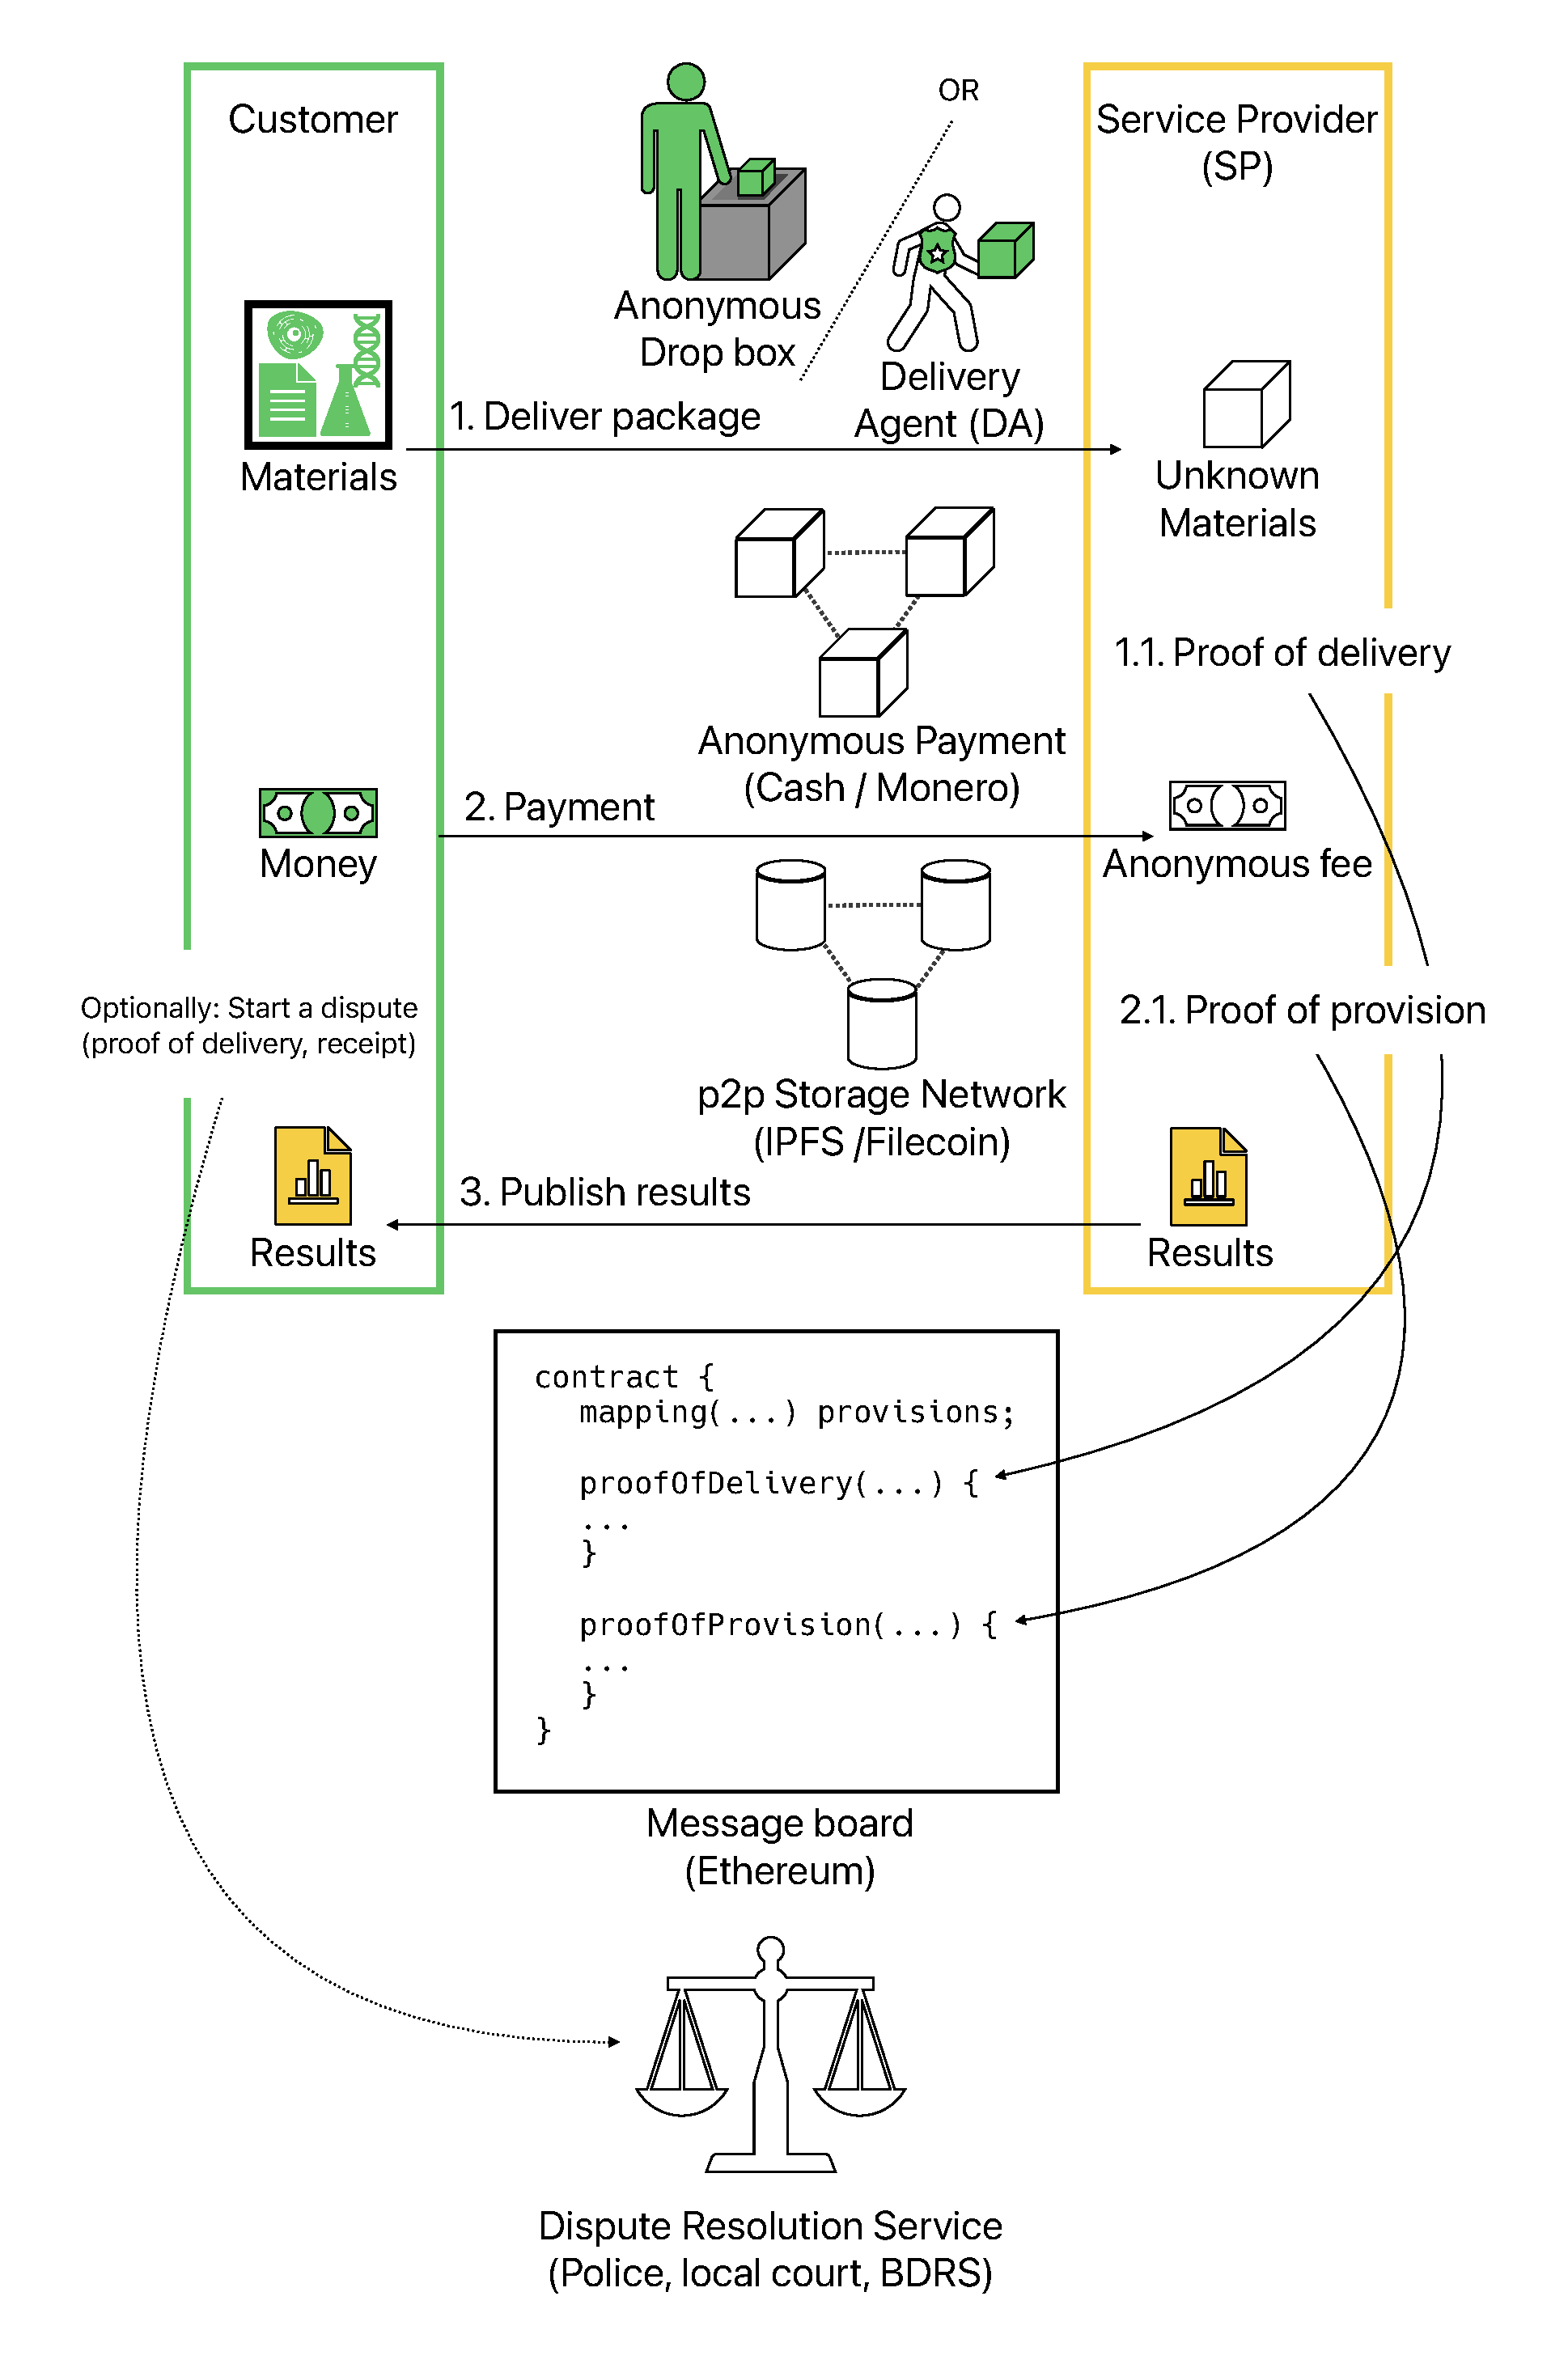
\includegraphics[width=\linewidth]{protocol-overview.pdf}
\centering
\caption{A simplified diagram of the protocol. The first step involves the delivery of the materials to the SP. The second step involves anonymous payment. The third step involves the delivery of the result to the customer. Each step is proven on the message board, protecting the fair party in a conflict situation.}

\label{fig:protocol-overview}
\end{figure}


\section{Related Works}\label{sec:related-works}
\begin{sloppypar}
This section reviews the main protocols for fair exchange, anonymity and physical delivery, highlighting their main features and differences.
\end{sloppypar}

The most common application of fair exchange protocols is in e-commerce. In a typical transaction, a seller and a customer exchange money for a physical product.
To protect themselves, the seller wants to receive the funds before sending the product, while the customer wants to receive the product before paying.
The fairness of the protocol should ensure that either both parties receive the goods or neither receives anything.
Early systems, such as those by Zhang et al. (2006)\cite{zhangPracticalFairExchangeEPayment2006} and Mohammedalaraj (2012)\cite{mohammedalarajFairnessPhysicalProducts2012}, introduced Trusted Third Parties (TTPs) and Delivery Agents (DAs) to ensure fairness and relied on strong assumptions about non-collusion and resilient communication channels.

\begin{sloppypar}
Protocols such as those proposed by Bîrjoveanu et al. (2015-2022)~\cite{birjoveanuAnonymityFairexchangeEcommerce2015, birjoveanuPreservingAnonymityFair2018, birjoveanuAnonymityComplexTransactions2019, birjoveanuFairExchangeECommerce2020, birjoveanuTwoPartyECommerceProtocols2022} focus on anonymity in transactions involving physical products. These protocols use TTPs, anonymous communication channels like Tor, and cryptographic techniques like blind signatures to ensure privacy and fairness. However, they rely on the existence of TTPs and secure, confidential transaction systems between banks.
\end{sloppypar}

Blockchain technology offers solutions to TTP dependency in fair exchange protocols. Hinarejos et al. (2019)\cite{hinarejosSolutionSecureCertified2019} demonstrated a blockchain-based protocol for certified email that replaces TTP with a decentralized, verifiable system. Themis (Meng et al., 2019)\cite{mengThemisDecentralizedEscrow2019} took this further by incorporating a decentralized dispute resolution mechanism, although it does not address anonymity.

Lelantos (Altawy et al., 2017)~\cite{altawyLelantosBlockchainBasedAnonymous2017} is a notable example of a blockchain-based system that provides anonymous physical delivery. It uses onion routing and smart contracts to ensure anonymity, although it only achieves pseudonymity and lacks a dispute resolution mechanism.

\paragraph{Comparison and our approach}

\begin{sloppypar}
We have only considered protocols that achieve fair exchange, as this is the fundamental feature of such protocols.
We also didn't focus on protocols for buying digital products, as they are not relevant to our use case. A more comprehensive analysis of such protocols is available in~\cite{birjoveanuTwoPartyECommerceProtocols2022}.
\end{sloppypar}

Altawy et al. 2017~\cite{altawyLelantosBlockchainBasedAnonymous2017} is a blockchain-based protocol that uses onion routing and anonymous blockchain interaction to provide anonymous physical delivery, assuming unlinkability between pseudonyms and real identities. However, it does not provide dispute resolution.
Hinarejos et al. 2019~\cite{hinarejosSolutionSecureCertified2019} is the simplest protocol that replaces TTP with blockchain. However, it does not take into account anonymity, disputes between parties, or the exchange of physical material.
Meng et al. 2019~\cite{mengThemisDecentralizedEscrow2019} improves on the previous protocol through a crowdsourced dispute resolution system. However, it does not consider anonymity.
Bîrjoveanu, 2022~\cite{birjoveanuTwoPartyECommerceProtocols2022} is the closest to our protocol, but it is based on strong assumptions, namely the existence of TTP, banks supporting confidential transactions with commit buffers, and maintaining a global list of coin serial numbers.

Our protocol differs from existing ones in that it focuses on anonymity and fair exchange without relying on TTPs or complex banking systems. It achieves anonymity by using either cash or privacy-preserving blockchains. In addition, our protocol does not require the customer to submit a transaction to the bulletin board, simplifying the transaction process while maintaining anonymity and fairness.

Table~\ref{tab:comparison} provides a summary of the key features and differences between the protocols discussed.

\begin{table*}
\centering
\newcommand{\YES}{\cellcolor{green!50}Yes}
\newcommand{\YESBUT}{\cellcolor{green!25}Yes*}
\newcommand{\ID}{\cellcolor{green!25}Identity}
\newcommand{\PSEUDO}{\cellcolor{green!35}Pseudonym}
\newcommand{\ANON}{\cellcolor{green!50}Anonymity}
\newcommand{\NO}{\cellcolor{red!50}No}
\newcommand{\TTP}{\cellcolor{red!50}TTP}
\newcommand{\OffTTP}{\cellcolor{orange!50}Offline TTP}
\newcommand{\OffBC}{\cellcolor{yellow!50}BC \& Offline TTP}
\newcommand{\BC}{\cellcolor{green!50}BC}
\caption{Comparison of related works. Category Definitions: \textit{E-commerce:} Secure online transactions for physical goods; \textit{Private Delivery System:} Methods ensuring fair and anonymous delivery of physical products; \textit{Certified email:} Secure exchange of certified electronic mail with proof of receipt; \textit{Digital escrow:} Decentralized escrow services for secure digital currency transactions. The notation \textit{Pseudonymity} means that the anonymity is based on the assumption that the pseudonym is not linked to the real identity; \textit{TTP} means that the protocol relies on a trusted third party in every transaction; \textit{Offline TTP} means that the protocol relies on a trusted third party only to resolve disputes; \textit{BC} means that the protocol uses a public blockchain; \textit{YES*} means that the protocol provides the feature but is based on strong or impractical assumptions.}
\label{tab:comparison}
\setlength{\tabcolsep}{3pt}

\begin{tabular}{ccccccc}

\noalign{\smallskip}\hline\noalign{\smallskip}
Protocol & Scenario & Fair exchange & Anonymity & Dispute resolution & Trust & Physical delivery \\
\noalign{\smallskip}\hline\noalign{\smallskip}
Zhang et al. \cite{zhangPracticalFairExchangeEPayment2006} (2006) & E-commerce & \YES & \YESBUT & \YES & \TTP & \YES  \\
Alaraj et al.\cite{mohammedalarajFairnessPhysicalProducts2012} (2012) & E-commerce & \YESBUT & \NO & \YES & \OffTTP & \YES \\
Lelantos~\cite{altawyLelantosBlockchainBasedAnonymous2017} (2017) & Private Delivery System & \YES & \PSEUDO & \NO & \BC & \YES \\
Hinarejos et al.\cite{hinarejosSolutionSecureCertified2019} (2019) & Certified email & \YES & \NO & \NO & \BC & \NO \\
Themis~\cite{mengThemisDecentralizedEscrow2019} (2019) & Digital escrow & \YES & \NO & \YES & \BC & \NO \\
PPPDCP~\cite{birjoveanuTwoPartyECommerceProtocols2022} (2022) & E-commerce & \YES & \YES & \YES & \TTP & \YES \\
This paper & E-commerce & \YES & \YES & \YES & \OffBC & \YES \\
\noalign{\smallskip}\hline

\end{tabular}

\end{table*}


\section{Building Blocks}\label{sec:building-blocks}

\subsection{Physical Products}\label{sec:physical-products}
In the realm of fair exchange protocols involving physical materials, existing solutions often rely on trusted intermediaries~\cite{mohammedalarajFairnessPhysicalProducts2012, birjoveanuAnonymityFairexchangeEcommerce2015} or complex delivery systems~\cite{altawyLelantosBlockchainBasedAnonymous2017} to maintain anonymity. While these methods are effective, they can be cumbersome and less practical for certain use cases.

In our context, the process is reversed, as the physical materials are transferred from an anonymous customer to a publicly known service provider (SP). This unique setup allows for a simplification of the delivery process. We propose several methods to facilitate anonymous delivery without compromising the customer's personal information:

\begin{itemize}
    \item \textbf{SP's Drop Box:} Utilizing a secure drop box provided by the SP, where customers can leave their packages without revealing their identity.
    
    \item \textbf{Parcel Locker Services:} Leverage existing locker services (e.g. Amazon Locker, InPost) that provide a level of anonymity and security for package delivery.
    
    \item \textbf{Trusted Delivery Agent:} The customer can use a trusted individual or service to deliver the package to the SP, ensuring the customer's anonymity.
    
    \item \textbf{Postal Services:} Traditional postal services may be used, provided they do not require personal identification or return addresses that could compromise anonymity.
\end{itemize}

\subsection{Dispute Resolution System}
\label{sec:dispute-resolution}
\begin{sloppypar}
Disputes are common in transactions, and systems are needed to ensure that rules and laws are followed. Traditionally, this has involved legal contracts and law enforcement. With blockchain technology, smart contracts offer a new way by putting the details of a contract into code and enforcing it through a consensus mechanism.~\cite{allenGovernanceBlockchainDispute2019,lingwallShouldCodeBe2019}.
\end{sloppypar}

\begin{sloppypar}
One challenge with blockchain is dealing with external information, which is where \textit{oracles} come in. They feed real-world data into the blockchain~\cite{breidenbachChainlinkNextSteps2021}. This is important for dispute resolution systems like Kleros~\cite{bergollaKlerosSociolegalCase2022, nappertDecentralizedJusticeReinventing2020, gudkovCrowdArbitrationBlockchain2020} or Themis~\cite{mengThemisDecentralizedEscrow2019}, which use decentralized networks to make fair decisions. Such arbitration services employ a pool of local experts who would
In the event of a dispute, they would examine the smart contract and all the evidence to provide verdicts back to the blockchain. The SP would be required to lock a certain amount of funds into the protocol, which would be cut in the event of misbehaviour. However, these systems may struggle with complex disputes that require specialised knowledge and privacy.
\end{sloppypar}

Our protocol takes a more traditional approach. It uses the blockchain to keep track of evidence, but relies on local legal systems (such as police or courts) to resolve disputes. In this way, we balance the use of technology with the need for detailed understanding in complicated service disputes. We talk more about exploring decentralized, partially automated systems in Section~\ref{sec:decentralised-justice}.

\subsection{Fairness}\label{fairness}
In our protocol, disputes are resolved by providing evidence to judicial authorities (police or courts). As the customer remains anonymous, the SP cannot initiate a dispute due to the inability to identify the customer. Our protocol is designed to favour the SP who adheres to the protocol, thus eliminating the need to initiate disputes. Conversely, customers can initiate disputes, but only misbehavior by the SP will result in a successful claim.

We outline three key pieces of evidence for dispute resolution:

\begin{enumerate}
  \item \textbf{Proof of Delivery ($\textrm{PoD}$)}: Issued by the SP to confirm that the customer has delivered a complete package in accordance with the SP's requirements. The detailed definition is given in Section~\ref{proof-of-delivery}.
  
  \item \textbf{Payment $\textrm{receipt}$}: This confirms that the customer has paid for the service. Its format varies depending on the payment method (cryptocurrency or cash) and is discussed further in Section~\ref{payment-for-services}.
  
  \item \textbf{Proof of Provision ($\textrm{PoP}$)}: This shows that the SP has published the service result at a certain time, thus protecting the SP against unjustified disputes from the customer. The detailed definition is given in Section~\ref{proof-of-provision}.
\end{enumerate}

\subsection{Message Board}\label{sec:message-board}
The platform for issuing and publishing these proofs is a critical aspect of the protocol. Known by various names such as bulletin board~\cite{achenbachImprovedCoercionresistantElectronic2015}, trusted timestamping~\cite{gippDecentralizedTrustedTimestamping2015}, or message board~\cite{hinarejosSolutionSecureCertified2019}, this platform serves as a decentralized, public ledger that securely timestamps and records each proof. By using blockchain technology, the platform ensures that the proofs are tamper-proof and verifiable by any third party, including judicial authorities.

This approach of using a decentralized message board to publish proofs has several advantages:
\begin{itemize}
  \item It creates an immutable record of the actions and agreements between the anonymous customer and the service provider.
  \item It allows transparent verification of the timeline of events, which is critical for dispute resolution.
\item It provides a universally accessible platform for verifying the authenticity and integrity of transaction-related proofs.
\end{itemize}

The protocol is designed to be adaptable, allowing for implementation with any decentralized technology capable of providing a message board service and supporting subscription to proofs from specific addresses.

\begin{sloppypar}
The choice between permissioned and permissionless blockchain touches on an ideological dispute about freedom and trust. The use of permissioned blockchain is recommended in domain-specific applications, such as closed consortia between distrustful parties. All the referenced protocols we've found use a public blockchain, suggesting that the fair exchange problem is allegedly not one of them. The public blockchain offers the irreplaceable qualities of total decentralisation, transparency, openness, no infrastructure maintenance costs (only transaction costs) and a different but arguably higher level of security (for networks with a high number of validators). In addition, protocols designed for public blockchains have a higher degree of generality and can be implemented in any private or permissioned blockchain. Therefore, for the rest of the paper, we only consider public networks.
\end{sloppypar}

\subsection{Anonymity, Pseudonymity, and Confidentiality}\label{sec:pseudo-anon}

\begin{sloppypar}
Privacy, a multifaceted concept in social sciences, is often ambiguously defined~\cite{smithInformationPrivacyResearch2011}. In our context, we focus on more concrete aspects: confidentiality, anonymity and pseudonymity.
\end{sloppypar}

\textbf{Confidentiality} refers to the ability to conceal the details of actions within a system. A system guarantees confidentiality if observers can only ascertain that an action occurred, without additional information.

\textbf{Anonymity} involves hiding one's identity within a system. It's the inability to link actions to a user's identity. Anonymity is a spectrum, quantifiable by \textit{k}-anonymity~\cite{sweeneyKanonymityModelProtecting2002}, where a user is \textit{k}-anonymous if their actions are indistinguishable from \textit{k}-1 other users. The larger the \textit{k}, the greater the anonymity.

\begin{sloppypar}
\textbf{Pseudonymity} differs from anonymity. Users operate under pseudonyms, and while actions can be linked to these pseudonyms, the system remains anonymous as long as the real identities behind these pseudonyms are concealed. However, this assumption is challenging due to KYC (Know Your Customer) and AML (Anti Money Laundering) regulations, which require users to reveal their real identities to cryptocurrency exchanges or other on-ramping services. This exposure of users' privacy to government agencies, malicious insiders, and cybercriminals complicates the maintenance of true anonymity and raises concerns about transaction analysis~\cite{androulakiEvaluatingUserPrivacy2013, oberStructureAnonymityBitcoin2013}.

Figure~\ref{fig:anonymity-diagram} illustrates these concepts. Alice, wanting anonymity, controls two addresses. The first address's link to her identity is compromised, but the second remains anonymous. Her actions from these addresses demonstrate the nuances of confidentiality and anonymity.
\end{sloppypar}

In the realm of blockchain technologies, the concepts of anonymity and confidentiality are achieved through different mechanisms, depending on whether the blockchain is privacy-preserving or not. We outline these differences below:

\begin{sloppypar}
\begin{enumerate}
    \item \textbf{Privacy preserving blockchains:} These blockchains inherently support both anonymity and confidentiality through advanced cryptographic techniques, ensuring that both user identities and transaction details are obscured. Examples include \textbf{Monero}, which uses ring signatures and bulletproofs~\cite{vansaberhagenCryptoNote2013, noetherRingSignatureConfidential2015, bunzBulletproofsShortProofs2018}, \textbf{ZCash}, which uses zkSNARKs for private transactions~\cite{ben-sassonZerocashDecentralizedAnonymous2014}, and \textbf{Grin} and \textbf{IronFish}, which use Mimblewimble and the Sapling protocol respectively~\cite{jedusorMIMBLEWIMBLE2016,fuchsbauerAggregateCashSystems2019, hopwoodZcashSaplingProtocol2022, ironfishPrivateAnonymousEasy}.
    \item \textbf{Non-privacy preserving blockchains:} These blockchains, such as Bitcoin and Ethereum, do not natively support strong privacy features. However, anonymity can be enhanced through the use of mixers and other privacy tools. Examples include \textbf{Tornado Cash} (Ethereum), which implements zkSNARKs and MiMC for enhanced privacy~\cite{grothSizePairingbasedNoninteractive2016,pertsevTornadoCashPrivacy2019}, and \textbf{Wasabi Wallet} (Bitcoin), which uses CoinJoin to mix transactions~\cite{maxwellCoinJoinBitcoinPrivacy2013,wasabiwalletBitcoinPrivacyWallet}.
\end{enumerate}
\end{sloppypar}


\begin{figure}[h!]
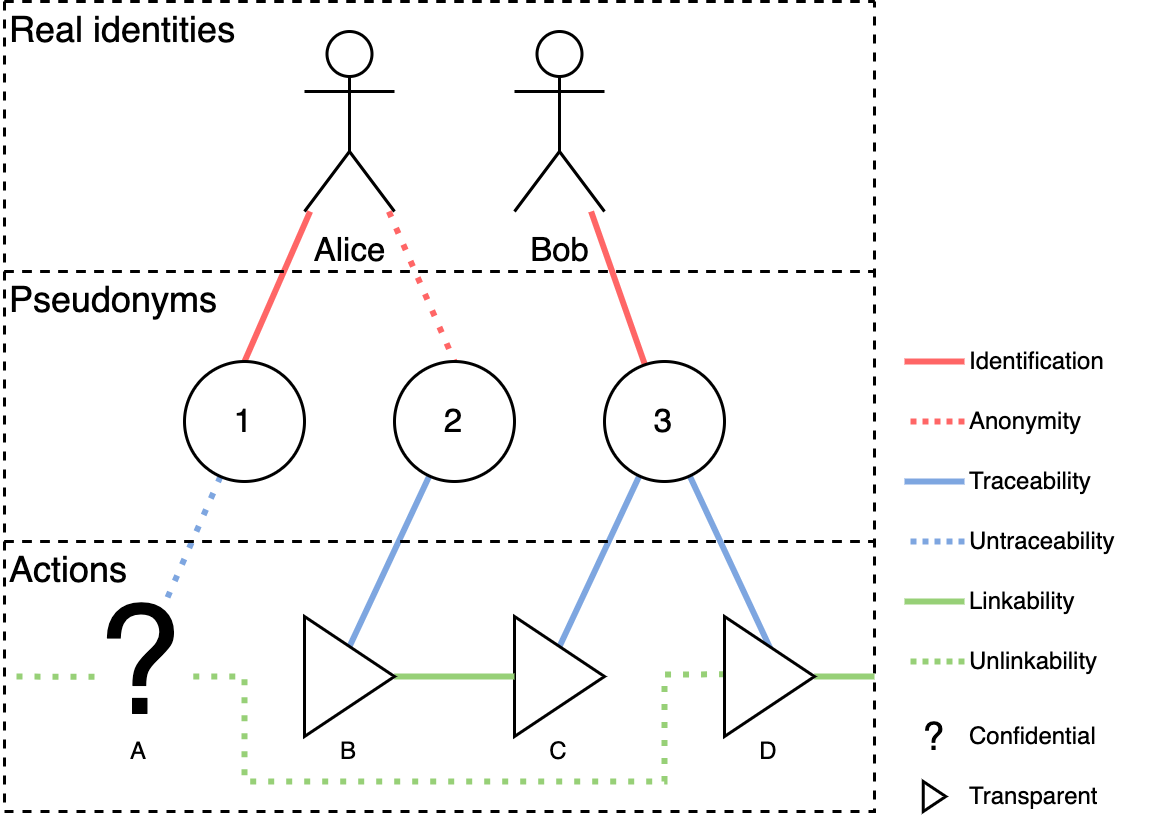
\includegraphics[width=\linewidth]{anonymity-diagram.png}
\centering
\caption{Consider a scenario where Alice is an anonymous customer and Bob is a public service provider (SP). Alice controls two addresses, labelled 1 and 2. The link (shown as a red line) between Alice's real identity and address 1 has been compromised, allowing identification. However, the link to address 2 remains unknown, preserving anonymity. Alice performs two actions, A and B. Action A is from the compromised address 1, while action B is from the anonymous address 2. Action A is confidential, meaning that despite the compromised pseudonym, the nature of the action remains undisclosed. Action B is transparent, but it cannot be linked to Alice as long as the connection to pseudonym 2 remains hidden.}
\label{fig:anonymity-diagram}
\end{figure}

\subsection{Paying for services}\label{payment-for-services}

\begin{sloppypar}
In transactions between customers and service providers (SPs), it is essential to establish a unique link between the payment and the corresponding transaction in order to prevent the reuse of a payment for multiple transactions. This link can be established in various ways depending on the cryptocurrency used:
\end{sloppypar}

\begin{sloppypar}
\begin{itemize}
    \item \textbf{Separate address:} Each transaction uses a unique address associated with it. These addresses can be generated using Hierarchical Deterministic Wallets~\cite{wuilleBIP32HierarchicalDeterministic2012} and published on the message board to ensure non-repudiation.
    \item \textbf{Memo:} Payments are sent to a single SP account but contain an extra field called ``memo'' filled with the unique identifier $\textrm{provisionID}$.
\end{itemize}
\end{sloppypar}

Any payment that contains $\textrm{provisionID}$ in the memo or is sent to the specified address will be recognized as payment for the transaction. 


\begin{sloppypar}
In the event of a dispute, it is necessary to prove to the courts that the customer has paid for the transaction. While proving payment is straightforward in transparent and traceable blockchains, it becomes more complex in anonymous blockchains. Monero, for example, allows payments to be proven and verified through a dedicated API~\cite{moneroHowProvePayment}, and ZCash provides a mechanism known as Payment Disclosure~\cite{daviesIntroductionPaymentDisclosure2017}. We refer to this proof of payment as a \textit{payment receipt}.
\end{sloppypar}

\subsection{Storage Network}\label{storage-network}

Upon completion of the service, the Service Provider (SP) faces the challenge of delivering the result to the customer while maintaining the customer's anonymity. The customer who wishes to remain anonymous cannot reveal their email address or IP address. In addition, the SP must prove that the result was delivered before a specified deadline, according to the concept of proof of existence discussed in section~\ref{sec:message-board}.

Even though the result does not contain private information (because the input data did not have it) we acknowledge the danger of storing on a distributed immutable record as blockchain.

\begin{sloppypar}
A common solution is to use a content addressable peer-to-peer storage network for data storage. This approach has been widely adopted in various applications~\cite{shahidBlockchainBasedAgriFoodSupply2020, wangAuditableProtocolsFair2019, chenImprovedP2PFile2017}. Specifically, data is stored on a network such as IPFS~\cite{benetIPFSContentAddressed2014}, and only the content identifier ($\mathrm{cid}$) that uniquely points to the content on IPFS is published on the blockchain.
\end{sloppypar}

Following this methodology, the SP encrypts the result using the encryption key provided by the client and uploads it to the IPFS network. 

The result is stored on public network so it is accessible to anyone with the cid address. However, the result is encrypted, so even if downloaded by third party it doesn't get access to the file unless it obtains the client's or SP's private key. 

To further increase anonymity, customers are advised to use standard techniques such as VPNs or proxies to hide their IP addresses.

\subsection{Provable Results Availability}

The demand-driven and opportunistic nature of IPFS storage means that the results may not be available indefinitely.

To ensure the availability of the results, we see two approaches. One involves fraud proofs, where an user which can not access the results invoke oracle service like Chainlink Request~\cite{breidenbachChainlinkNextSteps2021, ChainlinkMakeGET} which proves the content unavailability, and so pentalise the SP. 

The other approach is to integrate Filecoin as a decentralised pinning service to ensure the results are available for a defined period.

Filecoin enhances content availability on the IPFS network by economically penalizing the lack of proof of content storage~\cite{filecoinSlashing}.

The content availability is therefore economically guaranteed for the duration of the Filecoin contract.

Then, a file that is not further paid for in the Filecoin network is naturally deleted from the network as there is not incentive to keep it.

In this paper we explore the second approach and leave the first for future work.

\subsection{Separation of Concerns}\label{sec:separation-of-concerns}

\begin{sloppypar}
The protocol we propose could potentially use a single blockchain to fulfil three different roles: i) facilitating anonymous payments, ii) serving as a message board, and iii) acting as a storage network. However, while most blockchains can provide message board functionality, anonymous payments and a verifiable storage network are less common features and are often limited to specialized blockchains.

Rather than relying on a single blockchain to provide all functionalities, our protocol is designed to be flexible, allowing the use of separate blockchains for each specific role. This approach provides the freedom to choose the best available technology for each function. In the future, if a blockchain emerges that can efficiently handle multiple roles, it can be integrated into the protocol.

Based on the current state of blockchain technology, we identify the following platforms as suitable candidates for each role:
\begin{enumerate}
  \item \textbf{Anonymous payments:} Technologies such as Monero~\cite{vansaberhagenCryptoNote2013}, ZCash~\cite{ben-sassonZerocashDecentralizedAnonymous2014}, Grin~\cite{fuchsbauerAggregateCashSystems2019} and Tornado Cash~\cite{pertsevTornadoCashPrivacy2019} provide robust solutions for anonymous transactions.
  \item \textbf{Message Board:} Several platforms can be used for this purpose, including Open Timestamps~\cite{opentimestampsTimestampingProofStandard}, Stampery~\cite{crespoStamperyBlockchainTimestamping2017} and the Bitcoin blockchain with services like Proof of Existence~\cite{proofofexistenceWebApplicationProve} and Chainpoint~\cite{chainpointBlockchainProofAnchoring}. The Ethereum blockchain and other public blockchains that support attaching extra data to transactions are also viable options.
  \item \textbf{Storage Network:} For decentralized storage solutions, IPFS~\cite{benetIPFSContentAddressed2014}, Filecoin~\cite{protocollabsFilecoinDecentralizedStorage2017} and Ethereum's Swarm~\cite{teamSWARMStorageCommunication2021} are among the leading technologies.
\end{enumerate}
\end{sloppypar}

\section{The Protocol}\label{sec:protocol}
This section outlines an abstract protocol for anonymous service provisioning that is designed to be technology agnostic. It specifies the requirements for each role, allowing developers flexibility in technology choice. Implementation details and experimental validation of this protocol are discussed in Section~\ref{sec:experiments}.

\subsection{Assumptions}
The protocol is based on several key assumptions, each critical to its functionality and security:

\begin{itemize}
  \item \textbf{Cryptography and Public Key Infrastructure (PKI)}:
  \begin{itemize}
      \item The service provider (SP) has a key pair consisting of a secret key ($\mathrm{sk}_\mathrm{SP}$) and a publicly known public key ($\mathrm{pk}_\mathrm{SP}$).
      \item Digital signatures created by the SP ($\mathrm{sig}_{\mathrm{sk}_\mathrm{SP}}$) can be verified using the public $\mathrm{pk}_\mathrm{SP}$.
      \item The customer remains anonymous and does not require a publicly known key pair, thus ensuring their privacy and anonymity in the protocol.
      
    \begin{sloppypar}
      \item Both parties use standard symmetric encryption ($\mathrm{E}_\mathrm{key}(\cdot)$) and decryption ($\mathrm{D}_\mathrm{key}(\cdot)$) methods.
    \end{sloppypar}
\end{itemize}

\item \textbf{Service Provider (SP) Requirements}:
  \begin{itemize}
      \item The SP is willing to accept packages from unidentified customers.
      \item Payments are accepted in cash or anonymous cryptocurrencies, as detailed in Section~\ref{payment-for-services}.
   \end{itemize}
  
\item \textbf{Anonymous Payments Blockchain}:
  \begin{itemize}
      \item Facilitates anonymous transactions that are untraceable and ideally unlinkable.
      \item Allows transactions to be uniquely identified through dedicated addresses, memo fields or similar mechanisms (see Section~\ref{payment-for-services}).
  \end{itemize}

\item \textbf{Message Board}:
  \begin{itemize}
      \item Capable of handling transaction sizes up to $\mathrm{PoD}$ and $\mathrm{PoP}$.
  \end{itemize}

\item \textbf{Storage Network}:
  \begin{itemize}
      \item Enables content to be retrieved using a content identifier ($\mathrm{cid}$), typically a hash of the content.
      \item Ensures anonymous access to content.
      \item Guarantees that the content will be available for an agreed period of time.
  \end{itemize}
  
    
\item \textbf{Dispute Resolution Service}:
    \begin{itemize}
        \item Recognizes $\mathrm{PoD}$ (Proof of Delivery), $\mathrm{PoP}$ (Proof of Provision), and payment receipts as valid evidence in disputes (see Section~\ref{fairness}).
    \end{itemize}
\end{itemize}

\subsection{Messages}\label{messages}
This subsection details the messages exchanged between the parties in the protocol.

\vspace{5mm}

\noindent \textbf{Package}\label{package} is a physical container prepared by the customer containing all the $\mathrm{materials}$ required by the SP to provide the service.
\begin{equation}
\mathrm{pkg} \equiv (\mathrm{materials}, \mathrm{provisionID}, \mathrm{pk_C})
\end{equation}
where:
\begin{itemize}
\item $\mathrm{materials}$ - Materials required for the service provision, such as biological samples, legal documents or other relevant items.
\item $\mathrm{provisionID}$ - A unique identifier generated by the customer to anonymously track the provision through all protocol steps.
\item $\mathrm{pk_C}$ - The customer's public key for encrypting results to be published to the public storage network.
\end{itemize}

\noindent \textbf{Proof of Delivery ($\mathrm{PoD}$)}\label{proof-of-delivery} confirms the correct delivery of the package to the SP and its acceptance.

It is also an agreement between the customer and the SP as it contains the description of the expected item~\footnote{We follow the assumption from~\cite{asokanFairnessElectronicCommerce1998} that there exists a string that describes the desired item in "sufficient" detail so that during the dispute the arbitrator can decide whether the provided result is as agreed.}, agreed deadlines for actions and a payment method.
\begin{eqnarray}
\mathrm{PoD} & \equiv & (\begin{array}[t]{l}\mathrm{pk_C}, \mathrm{provisionID},    \mathrm{itemDescription}, \\\\ 
\mathrm{paymentAddress}, \mathrm{T}_\mathrm{issue}, \mathrm{T}_\mathrm{pay}, \mathrm{T}_\mathrm{provide}, \mathrm{sig}_\mathrm{SP} \; )\end{array}
\end{eqnarray}
where:
\begin{itemize}
\item $\mathrm{pk_C}$ - Customer's public key.
\item $\mathrm{provisionID}$ - Unique transaction identifier.
\item $\mathrm{itemDescription}$ - Hash of the description of the expected item.
\item $\mathrm{paymentAddress}$ - SP's anonymous payment address.

\item $\mathrm{T}_\mathrm{issue}$ - Time of $\mathrm{PoD}$ issuance.
\item $\mathrm{T}_\mathrm{pay}$ - Payment deadline.
\item $\mathrm{T}_\mathrm{provide}$ - Service provision deadline.
\item $\mathrm{sig}_\mathrm{SP}$ - SP's digital signature.
\end{itemize}

also:
\(\mathrm{T}_\mathrm{issue} \leq \mathrm{T}_\mathrm{pay} \leq \mathrm{T}_\mathrm{provide}\)

\noindent \textbf{Proof of Provision ($\mathrm{PoP}$)}\label{proof-of-provision} verifies the SP's publication of results at a specific time, protecting the SP against unjustified disputes.

The link between $\mathrm{PoP}$ and the results is made by the content identifier ($\mathrm{cid}$), which uniquely identifies the results so that the result cannot be forged after the $\mathrm{PoP}$ has been published.
\begin{equation}
\mathrm{PoP} \equiv (\mathrm{cid}, \mathrm{provisionID}, \mathrm{sig}_\mathrm{SP})
\end{equation}

where:
\begin{itemize}
\item $\mathrm{cid}$ - Content identifier as specified in Section~\ref{storage-network}.
\item $\mathrm{provisionID}$ - Unique transaction identifier.
\item $\mathrm{sig}_\mathrm{SP}$ - SP's digital signature.
\end{itemize}

\noindent \textbf
{Payment-receipt}\label{payment-receipt} proves that the customer made the payment. Since the proof depends on a specific blockchain (see Section~\ref{payment-for-services}), we symbolically refer to it as $\mathrm{receipt}$.

\begin{sloppypar}
\noindent \textbf{Results}\label{results} are typically in PDF format, but any binary-encodable format acceptable for the storage network can be used, symbolically referred to as $\mathrm{results}$.
\end{sloppypar}

\noindent \textbf{Content Identifier (cid)}\label{content-identifier-cid} is a term from IPFS~\cite{ipfsContentIdentifiersCIDs}. However, the protocol allows for any secure and unique identifier for content referencing.

\subsection{Protocol Description}\label{protocol-description}

This section outlines each step of the protocol, also shown in Figure~\ref{fig:protocol-diagram}.

\begin{figure}[ht!]
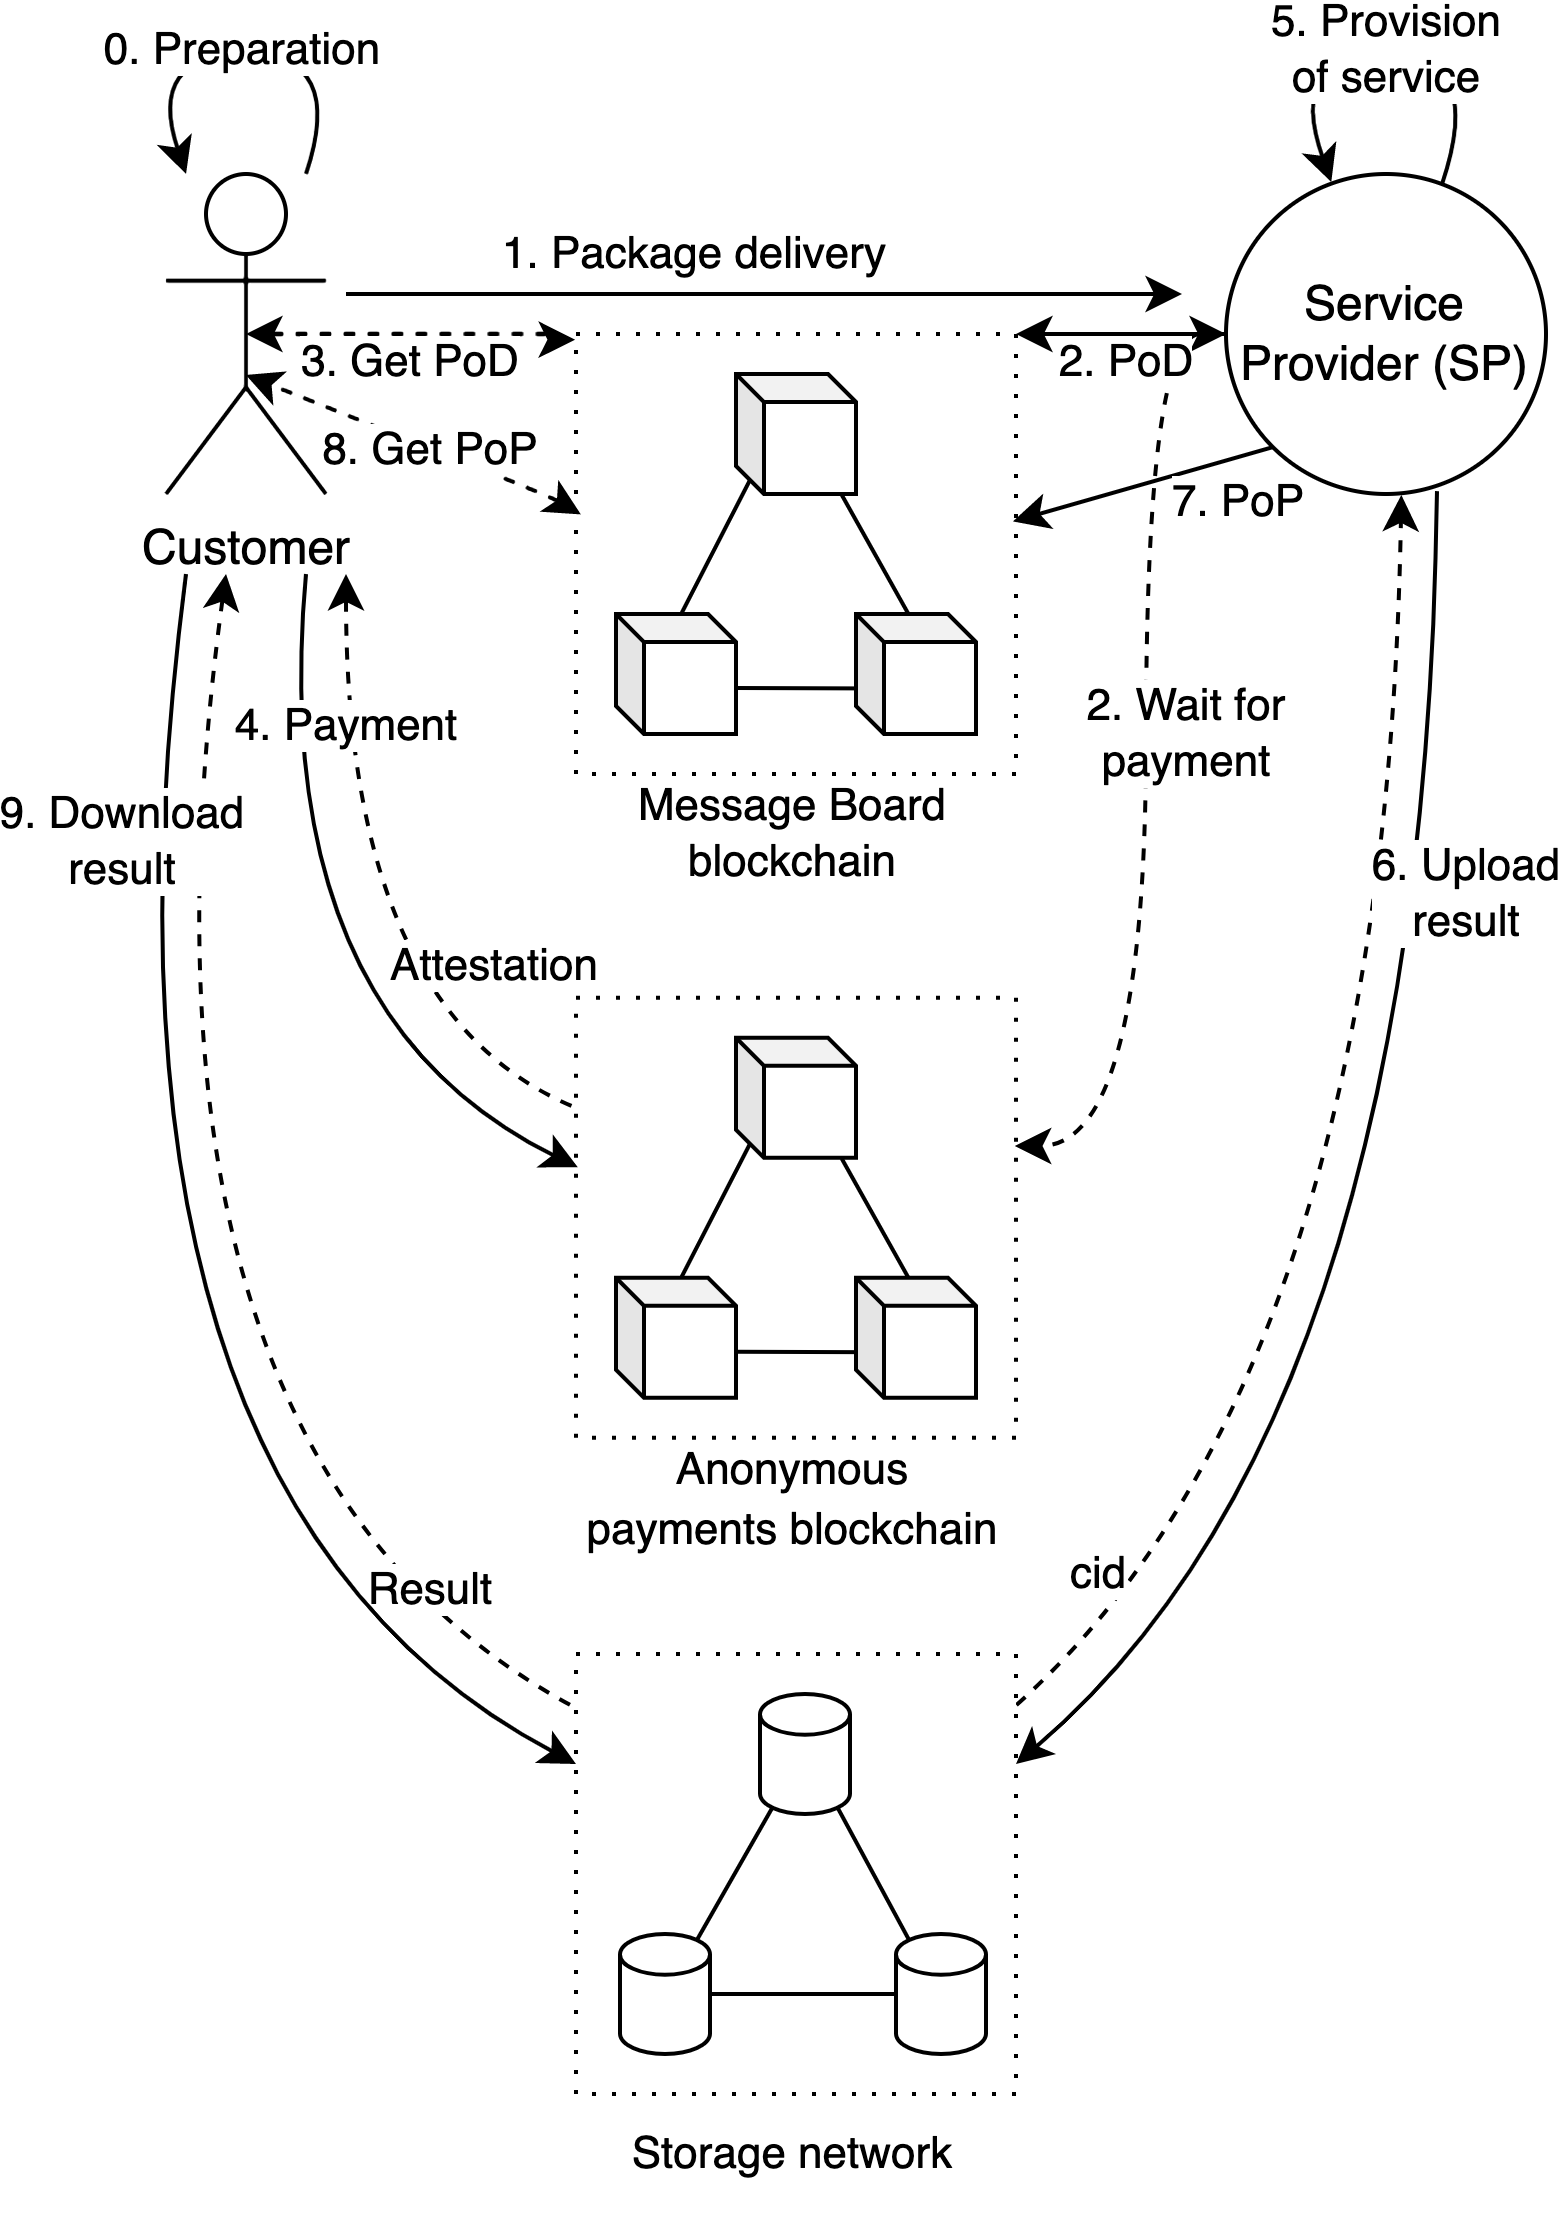
\includegraphics[width=\linewidth]{anonser-protocol.png}
\centering
\caption{Messages exchanged in the protocol. Solid arrows indicate requests and dashed arrows indicate responses.}
\label{fig:protocol-diagram}
\end{figure}

\noindent \textbf{Step 0. Preparation}\label{step-0-preparation}

The customer prepares the $\mathrm{materials}$ required by the SP, generates a random $\mathrm{provisionID}$, and a keypair $(\mathrm{sk_C},\mathrm{pk_C})$. The $\mathrm{provisionID}$ and $\mathrm{pk_C}$ are encoded as a QR code, attached to the $\mathrm{pkg}$. The $\mathrm{sk_C}$ is kept secret for decrypting the $\mathrm{result}$ later.

\noindent \textbf{Step 1. Package Delivery}\label{step-1-package-delivery}

The protocol initiates when the customer delivers $\mathrm{pkg}$ to the SP. The SP creates $\mathrm{PoD}$ with deadlines $\mathrm{T}_\mathrm{pay}$, $\mathrm{T}_\mathrm{provide}$, and $\mathrm{T}_\mathrm{issue}$. The $\mathrm{PoD}$ also specifies the description of the item $itemDescription$, and payment method (cash or blockchain address). The SP's digital signature $\mathrm{sig}_{\mathrm{sk}_\mathrm{SP}}$ on $\mathrm{PoD}$ ensures non-repudiation.

Symbolically: 
\[
\mathrm{PoD \gets delivery(pkg)}
\]

\noindent \textbf{Step 2. Proof of Delivery}\label{step-2-pod}

The SP publishes $\mathrm{PoD}$ on the message board, confirming receipt of $\mathrm{pkg}$. If not paid in cash, the SP awaits payment at the specified address in $\mathrm{PoD}$.

Symbolically: 
\[
\mathrm{publish(PoD)}
\]

The Algorithm~\ref{alg:proofOfDelivery} presents the process of processing the $\mathrm{PoD}$ and recording it on-chain.

\begin{algorithm}
\caption{Algorithm for Registering Proof of Delivery}
\label{alg:proofOfDelivery}
\begin{algorithmic}[1]
\Function{proofOfDelivery}{$pk_C$, $provisionId$, $itemDescription$, $paidInCash$, $paymentAddress$, $paymentWindow$, $provisionWindow$, $sig_{SP}$}
    \State Verify $sig_{SP}$
    \If{provisions[$pk_C$][$provisionId$] is not empty}
        \State \Return Error("Provision already exists")
    \EndIf

    \If{$paidInCash = \text{TRUE} \oplus paymentAddress$ is not empty}
        \State \Return Error("Pay in cash or specify paymentAddress")
    \EndIf
    
    \State $\mathrm{T}_\mathrm{issue} \gets$ block.timestamp
    \State $\mathrm{T}_\mathrm{pay} \gets \mathrm{T}_\mathrm{issue} + paymentWindow$
    \State $\mathrm{T}_\mathrm{provide} \gets \mathrm{T}_\mathrm{issue} + provisionWindow$

    \State $provision \gets \left\{ \mathrm{T}_\mathrm{issue}, \mathrm{T}_\mathrm{pay}, \mathrm{T}_\mathrm{provide} \right.$
    \State \hspace{\algorithmicindent}$\left. itemDescription, paidInCash, paymentAddress \right\}$
    \State provisions[$pk_C$][$provisionId$] $\gets provision$
\EndFunction
\end{algorithmic}
\end{algorithm}

\noindent \textbf{Step 3. Get Proof of Delivery}\label{step-3-get-pod}

The customer retrieves $\mathrm{PoD}$ from the message board and verifies payment details, $itemDescription$ and time windows ($\mathrm{T}_\mathrm{issue}$, $\mathrm{T}_\mathrm{pay}$, $\mathrm{T}_\mathrm{provide}$).

Symbolically: 
\[
\mathrm{PoD \gets get(pk_C, provisionID)}
\]

\noindent \textbf{Step 4. Payment}\label{step-4-payment}

If not paid in cash, the customer pays via the anonymous blockchain, receiving a $\mathrm{receipt}$.

Symbolically: 
\[
\mathrm{receipt \gets payment(paymentAddress)}
\]

\noindent \textbf{Step 5. Provision of Service}\label{step-5-provision-of-service} 

Upon payment confirmation, the SP begins service provision.

Symbolically: 
\[
\mathrm{result \gets provision(materials)}
\]

\noindent \textbf{Step 6. Upload Result}\label{step-6-upload-result}

The SP encrypts the $\mathrm{result}$ using $\mathrm{E_{DHKE(sk_{SP}, pk_C)}}$ and uploads it to the storage network, receiving a $\mathrm{cid}$.

Symbolically: 
\[
\mathrm{cid \gets upload(E_{DHKE(sk_{SP}, pk_C)}(result))}
\]

\noindent \textbf{Step 7. Proof of Provision}\label{step-7-proof-of-provision}

The SP publishes $\mathrm{PoP}$ on the message board, including $\mathrm{cid}$ and $\mathrm{provisionID}$.

Symbolically: 
\[
\mathrm{publish(PoP)}
\]

The Algorithm~\ref{alg:proofOfProvision} presents the process of processing the $\mathrm{PoP}$ and recording it on-chain.

\begin{algorithm}
\caption{Algorithm for Registering Proof of Provision}
\label{alg:proofOfProvision}
\begin{algorithmic}[1]
\Function{proofOfProvision}{$pk_C$, $provisionId$, $cid$, $sig_{SP}$}
    \State Verify $sig_{SP}$
    \State $provision \gets$ provisions[$pk_C$][$provisionId$]
    \If{not $provision$.exist}
        \State \Return Error("Provision must be created with proof of delivery first")
    \EndIf
    \State Update $provision$ with $\{cid\}$
    \State provisions[$pk_C$][$provisionId$] $\gets$ $provision$
\EndFunction
\end{algorithmic}
\end{algorithm}

\noindent \textbf{Step 8. Get Proof of Provision}\label{step-8-get-proof-of-provision}

The customer monitors the message board for the SP's $\mathrm{PoP}$.

Symbolically: 
\[
\mathrm{cid \gets get(pk_C, provisionID)}
\]

\noindent \textbf{Step 9. Download Result}\label{step-9-download-result}

The customer downloads and decrypts the $\mathrm{result}$ using $\mathrm{D_{DHKE(sk_C, pk_{SP})}}$.

Symbolically: 
\[
\mathrm{result \gets D_{DHKE(sk_C, pk_{SP})}(download(cid))}
\]

\section{Fair Exchange Analysis}\label{sec:fairness-analysis}

Fair exchange protocols involve two parties trading items with each other, where each party holds an item to trade and expects to receive a specific item in return. These protocols operate even when the parties do not necessarily trust each other. A key goal of fair exchange protocols is to ensure that a dishonest participant cannot exploit the situation to gain an advantage over an honest participant. Specifically, these protocols must meet the following requirements~\cite{asokanFairnessElectronicCommerce1998, liuFairnessCryptocurrencyPayments2018}:
\begin{enumerate}

    \item \textbf{R1, Fairness}: Fairness can be defined in two ways:\begin{itemize}
        \item \textbf{R1a Strong fairness}: Upon protocol completion, either both participants receive their desired items (successful exchange) or neither does (exchange fails).
        \begin{sloppypar}
        \item \textbf{R1b Weak fairness}: When strong fairness is not achievable, an honest participant can demonstrate to an external arbiter that the other party has received (or still can receive) the expected item.
        \end{sloppypar}
    \end{itemize}


    \item \textbf{R2, Timeliness}: An honest participant can be assured that the exchange will conclude (either successfully or unsuccessfully) within a specified timeframe, regardless of the other participant's behavior. At the end of the protocol, the outcome is final from the honest participant's perspective (e.g., the fairness ensured by the protocol remains consistent).
    
    \item \textbf{R3, Effectiveness}: The protocol guarantees successful completion of the exchange if both participants act correctly and agree to trade.

\end{enumerate}    


\subsection{Weak fairness}
Here we show that with the use of an external arbitrator (Dispute Resolution Service), either both parties receive their desired items at the end of the protocol, or neither receives anything. That is, the customer gets $result$ and the SP gets $payment$, or neither gets anything. This is how \textbf{R1b Weak Fairness} is achieved. 

First, we represent the protocol as an interactive non-cooperative game and analyse the strategic interactions between the service provider (SP) and the customer. We then show that successful completions result in both parties receiving desired items, and all unsuccessful completions result in both parties receiving nothing. We also extend the definition to include penalties for misbehaviour, which discourages frivolous or uncertain disputes.

\subsubsection{Model}\label{sec:fairness-model}
We define three distinct positions to represent the state of each party within the protocol:


\begin{itemize}
\item \textbf{Neutral Position ($\neutral{}$)}: The state of a party when no significant resources (money, time, effort) have been expended or acquired.
\item \textbf{Disadvantaged Position ($\minus{}$)}: The state of a party when it has invested resources without receiving a commensurate return, like a customer who has paid in advance for a service.
\item \textbf{Advantaged position ($\plus{}$)}: A scenario where stopping the transaction would result in a benefit to one party, e.g. where the SP has been paid but has not yet delivered the service.
\end{itemize}

The actions of each party are categorized as follows:

\begin{enumerate}
\item \textbf{Normal} ($\normal{}$): Those who adhere to the prescribed steps of the protocol.
\item \textbf{Abnormal} ($\abnormal{}$): Any deviation from the protocol's prescribed steps, such as sending irrelevant messages, skipping steps, or exceeding time limits.
\end{enumerate}

Additionally, the customer has the option to initiate a dispute at any protocol step, introducing another strategic layer:

\begin{enumerate}
\def\labelenumi{\arabic{enumi}.}
\item \textbf{Agree} ($\normal{}$ or $\abnormal{}$): The customer consents to the action and refrains from disputing.
\item \textbf{Start a dispute} ($\dispute{}$ or $\abdispute{}$): The customer opposes the action and initiates a dispute.
\end{enumerate}

\begin{sloppypar}
Consequently, our analysis needs to consider four possible $\mathrm{action} \in \{ \normal{}, \abnormal{}, \dispute{}, \abdispute{} \}$, for each $\mathrm{party \in \{C, SP\} }$, at every protocol step $\mathrm{step \in 1..9}$:
\end{sloppypar}

\begin{enumerate}
\item $\mathrm{\sigma_{step,party,\normal{}}}$: The outcome after adhering to the protocol with the other party acting normally.
\item $\mathrm{\sigma_{step,party,\dispute{}}}$: The outcome following a resolved dispute with the other party acting normally.
\item $\mathrm{\sigma_{step,party,\abnormal{}}}$: The outcome when no dispute is raised despite the other party's abnormal actions.
\item $\mathrm{\sigma_{step,party,\abdispute{}}}$: The outcome after a resolved dispute with the other party acting abnormally.
\end{enumerate}

\begin{sloppypar}
The protocol ends after the final step, if a dispute is initiated, or if a party fails to take the required action within the specified timeframe. Therefore, all positions except $\mathrm{\sigma_{step, party, n}}$ for $\mathrm{step} \in 1..8$ indicate the end of the protocol.
\end{sloppypar}

The anonymity of the customer prevents the SP from initiating a dispute. To address this, the protocol is designed in such a way that an SP who adheres to the protocol remains in an advantageous position, eliminating the incentive to dispute. Conversely, the customer can dispute at any time, but only proven misbehavior of the SP will result in a successful dispute. The Algorithm~\ref{alg:disputeResolution} presents the process of dispute resolution.

\begin{algorithm}
\caption{Algorithm for Dispute Resolution}
\label{alg:disputeResolution}
\begin{algorithmic}[1]
\Function{Dispute Resolution}{$pk_C$, $provisionId$, $receipt$, $result$}
    
    \State $provision$ $\gets$ $provisions$[$pk_C$][$provisionId$]
    \If{Time dispute}
    \State Verify $provision$.$paidInCash$ OR  (valid $receipt$ AND $receipt$.time < $provision$.$\mathrm{T}_\mathrm{pay}$)
    \State Verify not $provision$.$cid$ and $provision$.$provisionTime$ > $provision$.$\mathrm{T}_\mathrm{provide}$
    \State \Return The Customer wins the dispute because the SP has not provided the PoP on the agreed time.
    \EndIf
    \If{Result dispute}
        \State $provision$.$cid$ $\equiv$ $result$
        \State $provision$.$itemDescription$ $\not\equiv$ $result$
        \State \Return The Customer wins the dispute because the SP has not provided the desired result.
    \EndIf
\EndFunction
\end{algorithmic}
\end{algorithm}

% \begin{definition}[Weak Fairness] \label{def:fairness}
% Let $\mathrm{parties} = \{ C, SP \}$, $\mathrm{steps} = 1..9$, $\mathrm{actions} = \{ \normal{}, \abnormal{}, \dispute{}, \abdispute{} \}$, and 

% \begin{equation}
% M_{\sigma_\mathrm{s,p,a}} = 
% \begin{cases} 
% \{ \mathrm{\sigma_{s+1,p,\normal}}, \mathrm{\sigma_{s+1,p,\abnormal}}, \mathrm{\sigma_{s,p,\dispute}}, \mathrm{\sigma_{s,p,\abdispute}} \} & \text{if } s < 9, a = \normal{} \\
% \{ \mathrm{\sigma_{s,p,a}} \} & \text{otherwise} 
% \end{cases}
% \end{equation}
% represent the set of all possible positions a party $\mathrm{p}$ can move to at step $\mathrm{s}$ by taking action $\mathrm{a}$, from position $\sigma_\mathrm{s,p,a}$. The second case in $M_{\sigma_\mathrm{s,p,a}}$ represents the termination positions.

% A protocol is said to be fair if, at each step, both the customer and the service provider have the option to move to or remain in a non-disadvantaged position.

% \begin{equation}
% \forall_{\mathrm{p} \in \mathrm{parties}} \forall_{\mathrm{s} \in \mathrm{steps}} \forall_{\mathrm{a} \in \mathrm{actions}} \exists \sigma \in M_{\sigma_\mathrm{s, p, a}} \text{ such that } \sigma \neq -
% \end{equation}
% \end{definition}


\subsubsection{Assumptions}\label{sec:assumptions}

For the purpose of our analysis, we operate under the following assumptions:

\begin{enumerate}
\item Both parties start from a neutral position ($\neutral{}$), implying no initial advantage or disadvantage.
\item Upon successful completion of the transaction, both parties reach an advantageous position (\plus{}), indicating mutual benefit and motivation to initiate and complete the transaction.
\item The steps within the protocol are atomic, i.e. they are indivisible and have no intermediate states.
\item The protocol is unidirectional; actions taken cannot be reversed or undone.
\item The protocol can only be restarted by repeating the first step. Any repetition of subsequent steps is considered abnormal and will be disregarded. For example, a double payment does not change the course of the protocol.
\item Once the result of the service is published, it becomes available to the customer via the storage network.
\item A successful dispute resolution restores the disputing party to a neutral position ($\neutral{}$).
\item Losing a dispute incurs a penalty that exceeds any potential gain, resulting in a disadvantaged position (\minus{}). This discourages frivolous or uncertain disputes.
\item Both the customer and the SP are rational actors who prefer to move from a less advantageous to a more advantageous position. However, they may temporarily accept a less advantageous position if it leads to a subsequent advantageous state, as long as there is an escape route from the less advantageous position. Specifically, the client can initiate a dispute to move from a disadvantaged (\minus{}) to a neutral ($\neutral{}$) position if the SP fails to comply with the protocol.
\item The customer's materials, without personal information, have no value and the effort to deliver the package is considered minimal. Thus, the customer's first step does not lead to a disadvantaged position.
\item The cost of publishing the Proof of Delivery (PoD) is negligible and is offset by the customer's effort in delivering the package.
\end{enumerate}

\subsection{Proofs}\label{sec:proofs}

\begin{theorem}
The proposed protocol satisfies the security requirement of \textbf{R1b Weak fairness}.  
\end{theorem}

\begin{proof} 
The positions of each party after each action within our protocol are visually represented in Figure~\ref{fig:positions}. The detailed description of each step and the reasoning behind the outcomes is given in~\ref{app:proof-of-fairness}.

\begin{figure}[h!]
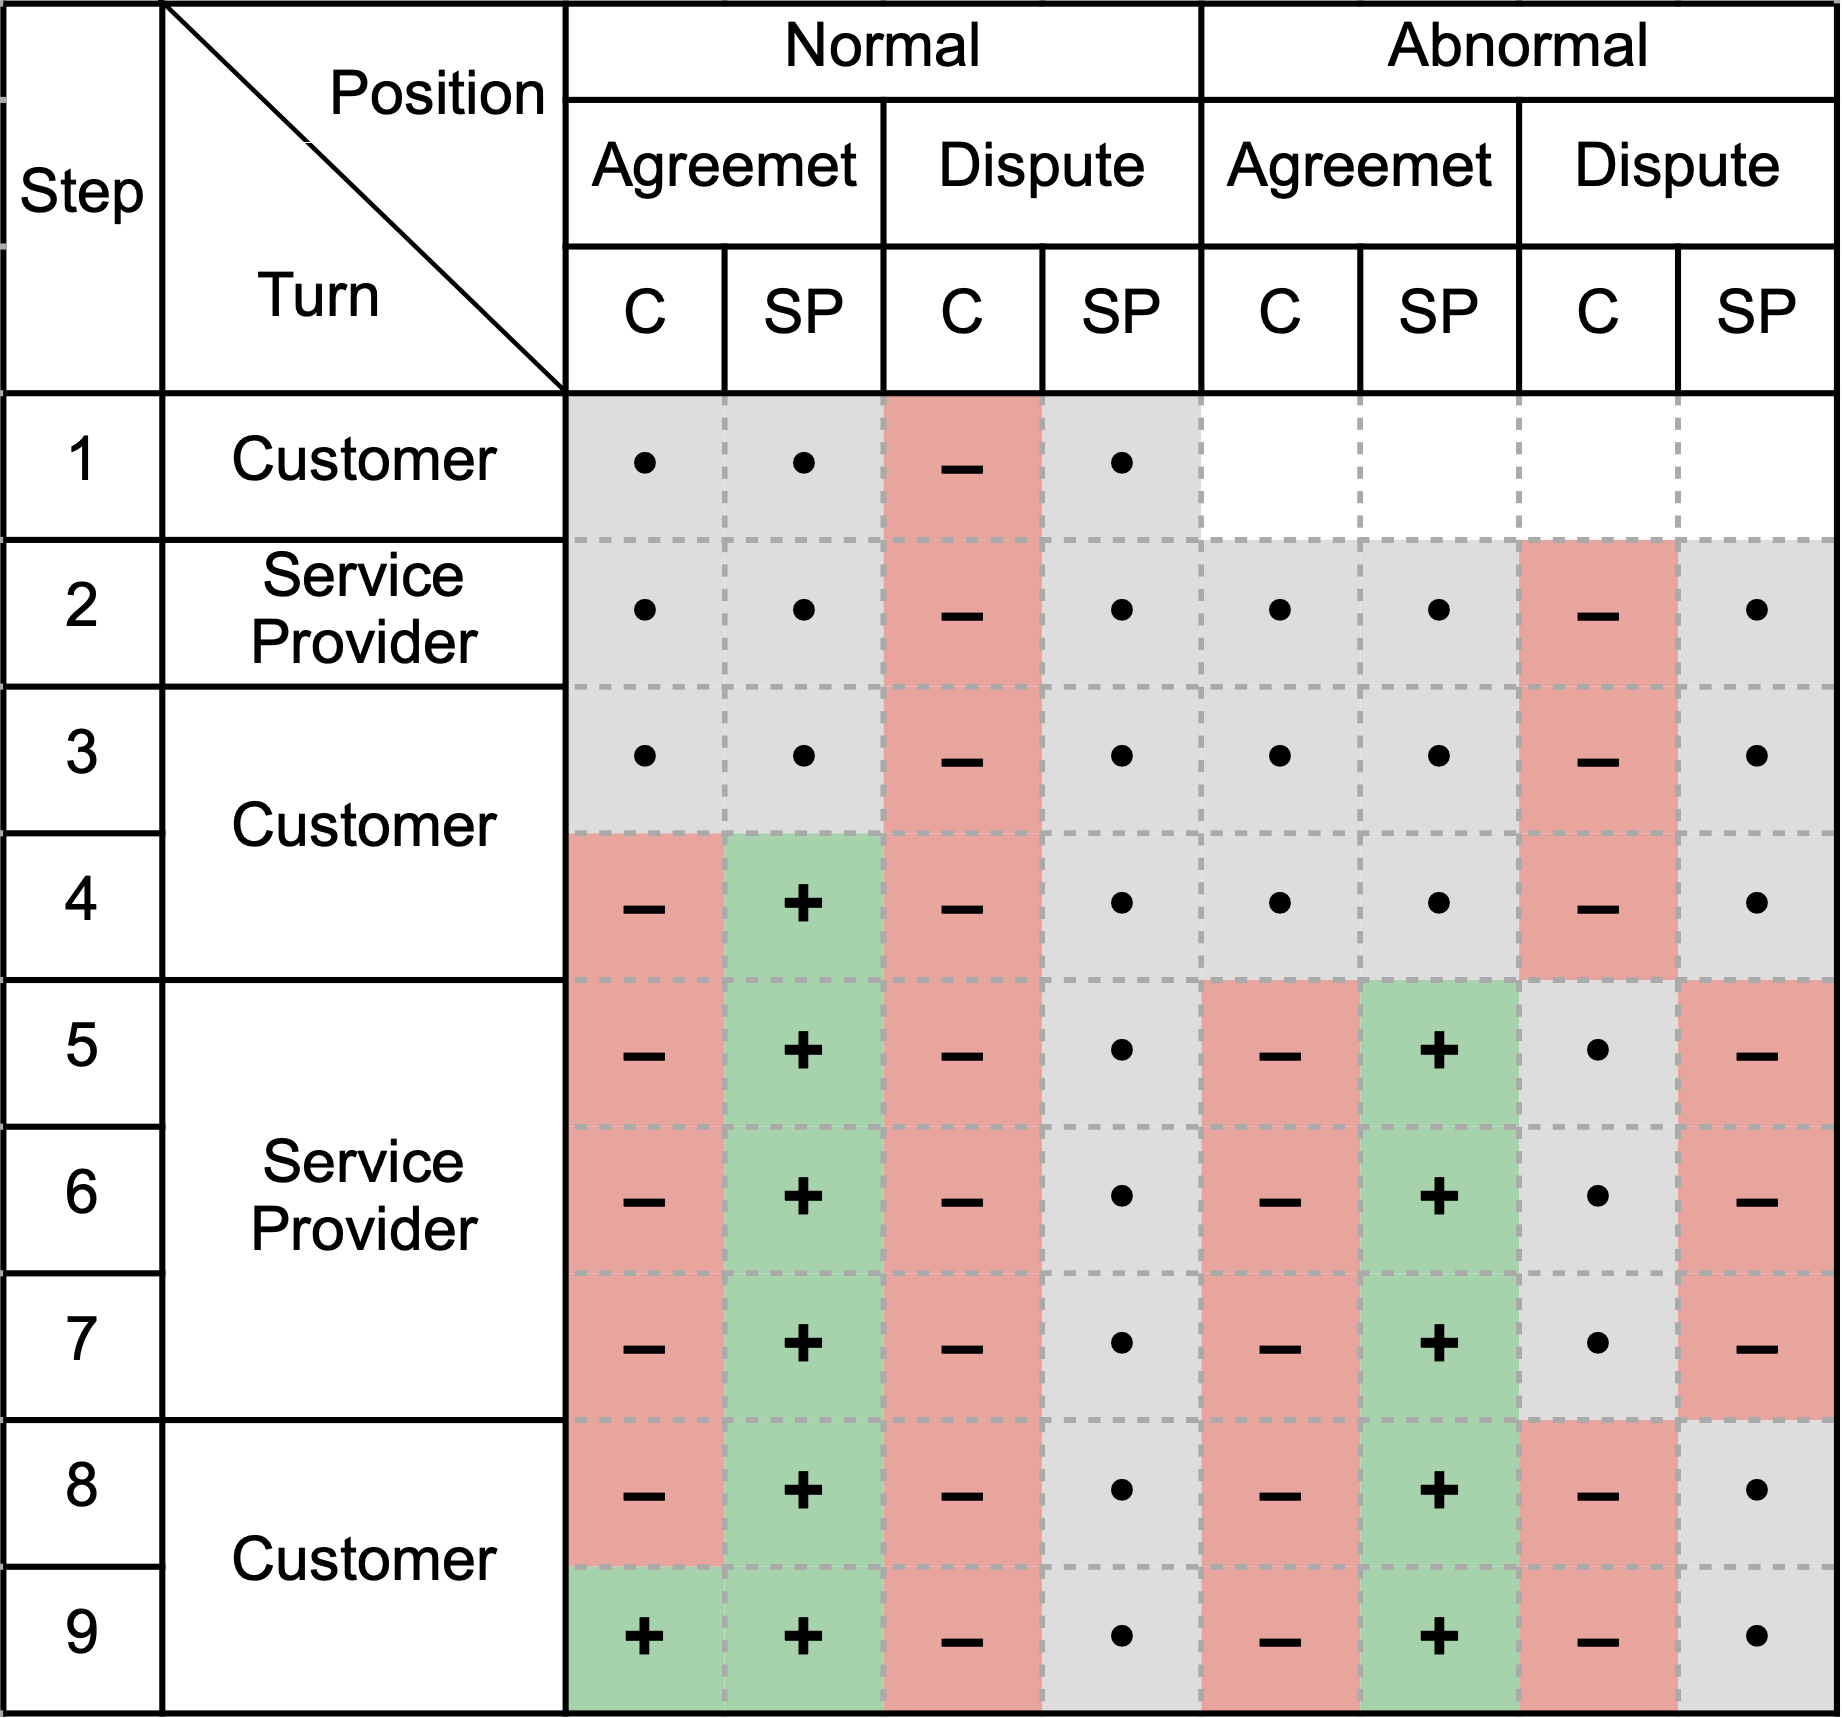
\includegraphics[width=\linewidth]{model.png}
\centering
\caption{Visual representation of the fairness of the protocol. This figure shows the outcomes for each party after various actions. The symbols used are $\neutral{}$ for a neutral outcome, \minus{} for a disadvantaged outcome, and \plus{} for an advantaged outcome. The order relation is defined as \minus{} < $\neutral{}$ < \plus{}.}
\label{fig:positions}
\end{figure}

Following the definition of \textbf{R1b Weak fairness} it's sufficient to show that, with the use of an external arbitrator (Dispute Resolution Service), the protocol completes either with both parties getting the desired items (advantaged positions), or neither does (neutral or disadvantaged).
The protocol (successfully) completes at the last normal agreement step ($\sigma_{9,n}$), and (unsuccessfully), after starting a dispute ($\sigma_{\dispute}$ or $\sigma_{\abdispute}$). 
We consider only honest (rational) customer, and so it will always starts a dispute after the SP misbehaves, and so it will never settle at abnormal agreement positions ($\sigma_{\abnormal}$, as that would be irrational.

\end{proof}


\begin{theorem}
The proposed protocol satisfies the security requirement of \textbf{R2, Timeliness}.  
\end{theorem}

\begin{proof} 

The timeliness of the protocol is achieved through the use of blockchain. Assuming an honest majority, the blockchain acts as a global, immutable and undeniable clock that timestamps every action and moves the protocol forward. Every step must be recorded on the blockchain, once the transaction is recorded it's undeniable.

Both parties agree to the timelines $\mathrm{T}_\mathrm{issue}$, $\mathrm{T}_\mathrm{pay}$, $\mathrm{T}_\mathrm{provide}$ and so any breach of the timelines is undeniably conclusive. The blockchain continuously creates blocks at a probabilistic rate. If a party hasn't completed its step within a time window, it can't publish a transaction in a previous block. Consequently, the protocol cannot move from a completed to an uncompleted state, nor can it hang in an uncompleted position, as the blocks produced move the parties' states out of the agreed timelines, thus fulfilling the \textbf{R2, Timeliness} requirement.
\end{proof}


% TODO: finish this train of thought
% TODO: The transaction actually can hang out if one party voliate and the other doesn't start a dispute. We would have to add a period of time where the dispute is 
% An honest participant can be assured that the exchange will conclude (either successfully or unsuccessfully) within a specified timeframe, regardless of the other participant's behavior. At the end of the protocol, the outcome is final from the honest participant's perspective (e.g., the fairness ensured by the protocol remains consistent).


\begin{figure}[h!]
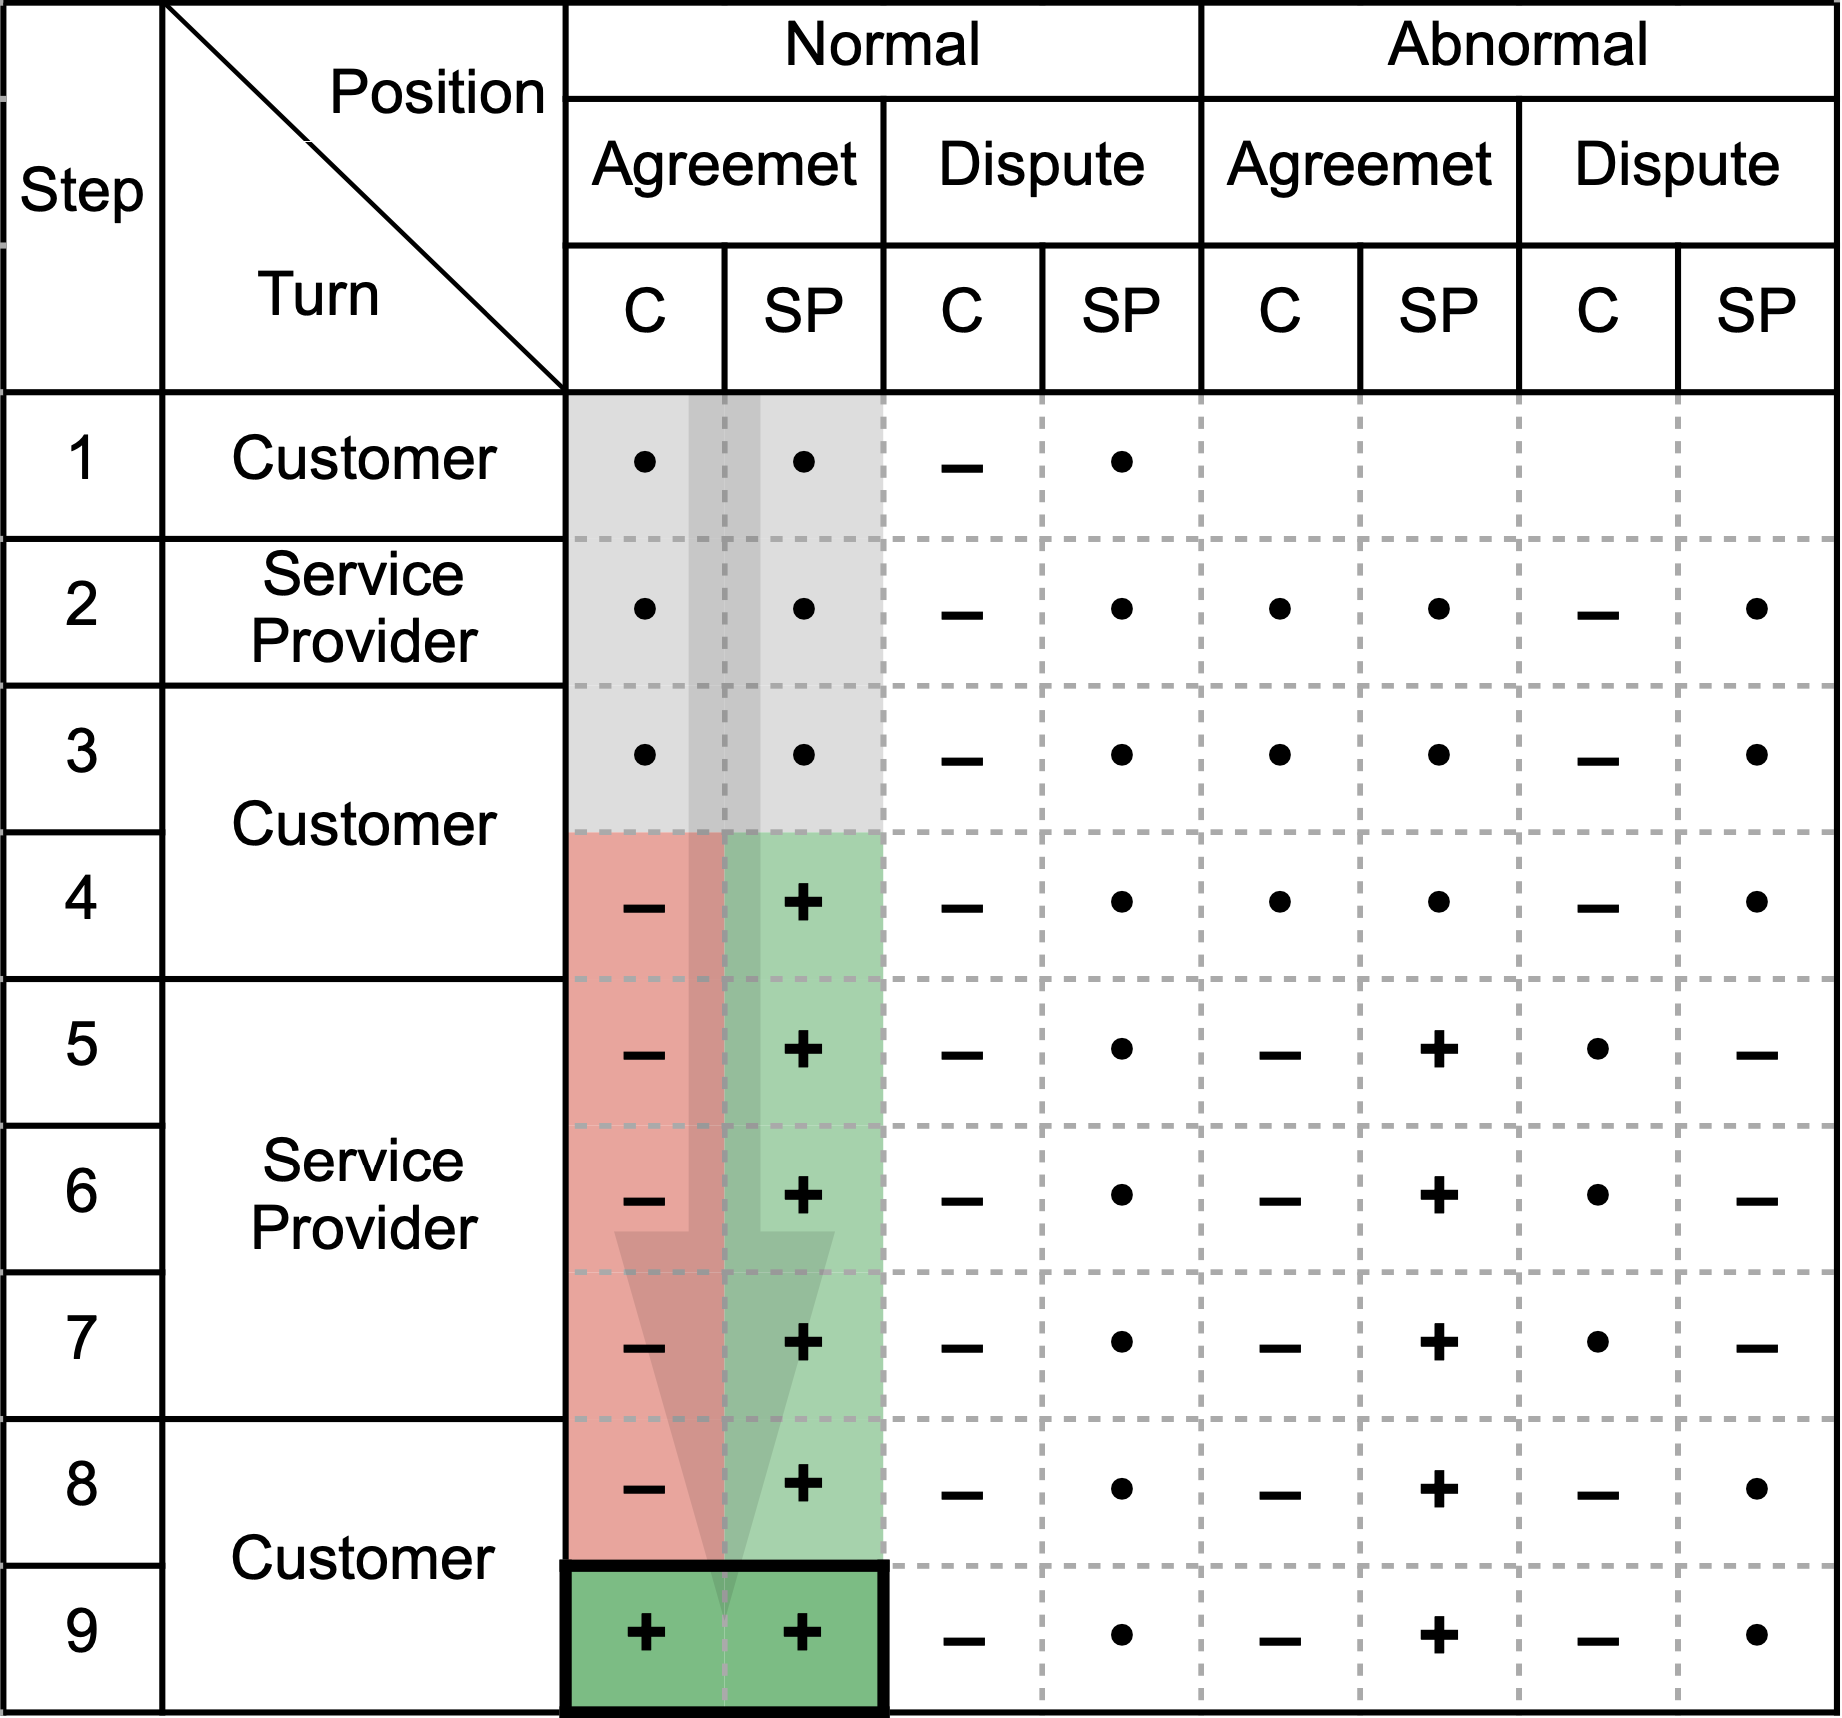
\includegraphics[width=\linewidth]{rational.png}
\centering
\caption{Transitions of positions in a scenario where both the customer and the SP adhere to the protocol.}
\label{fig:rational}
\end{figure}

\begin{theorem}
The proposed protocol satisfies the security requirement of \textbf{R2, Effectiveness}.  
\end{theorem}

The first scenario (Figure~\ref{fig:rational}) represents the rational and intended course of action, where both the client and the SP follow the protocol as designed. This scenario is crucial as it shows that parties who act correctly (normally and agreeably) will eventually succeed and thus \textbf{R3, Effectiveness} is achieved.

\subsection{Dispute scenario}\label{sec:example-scenarios}

\begin{figure}[h!]
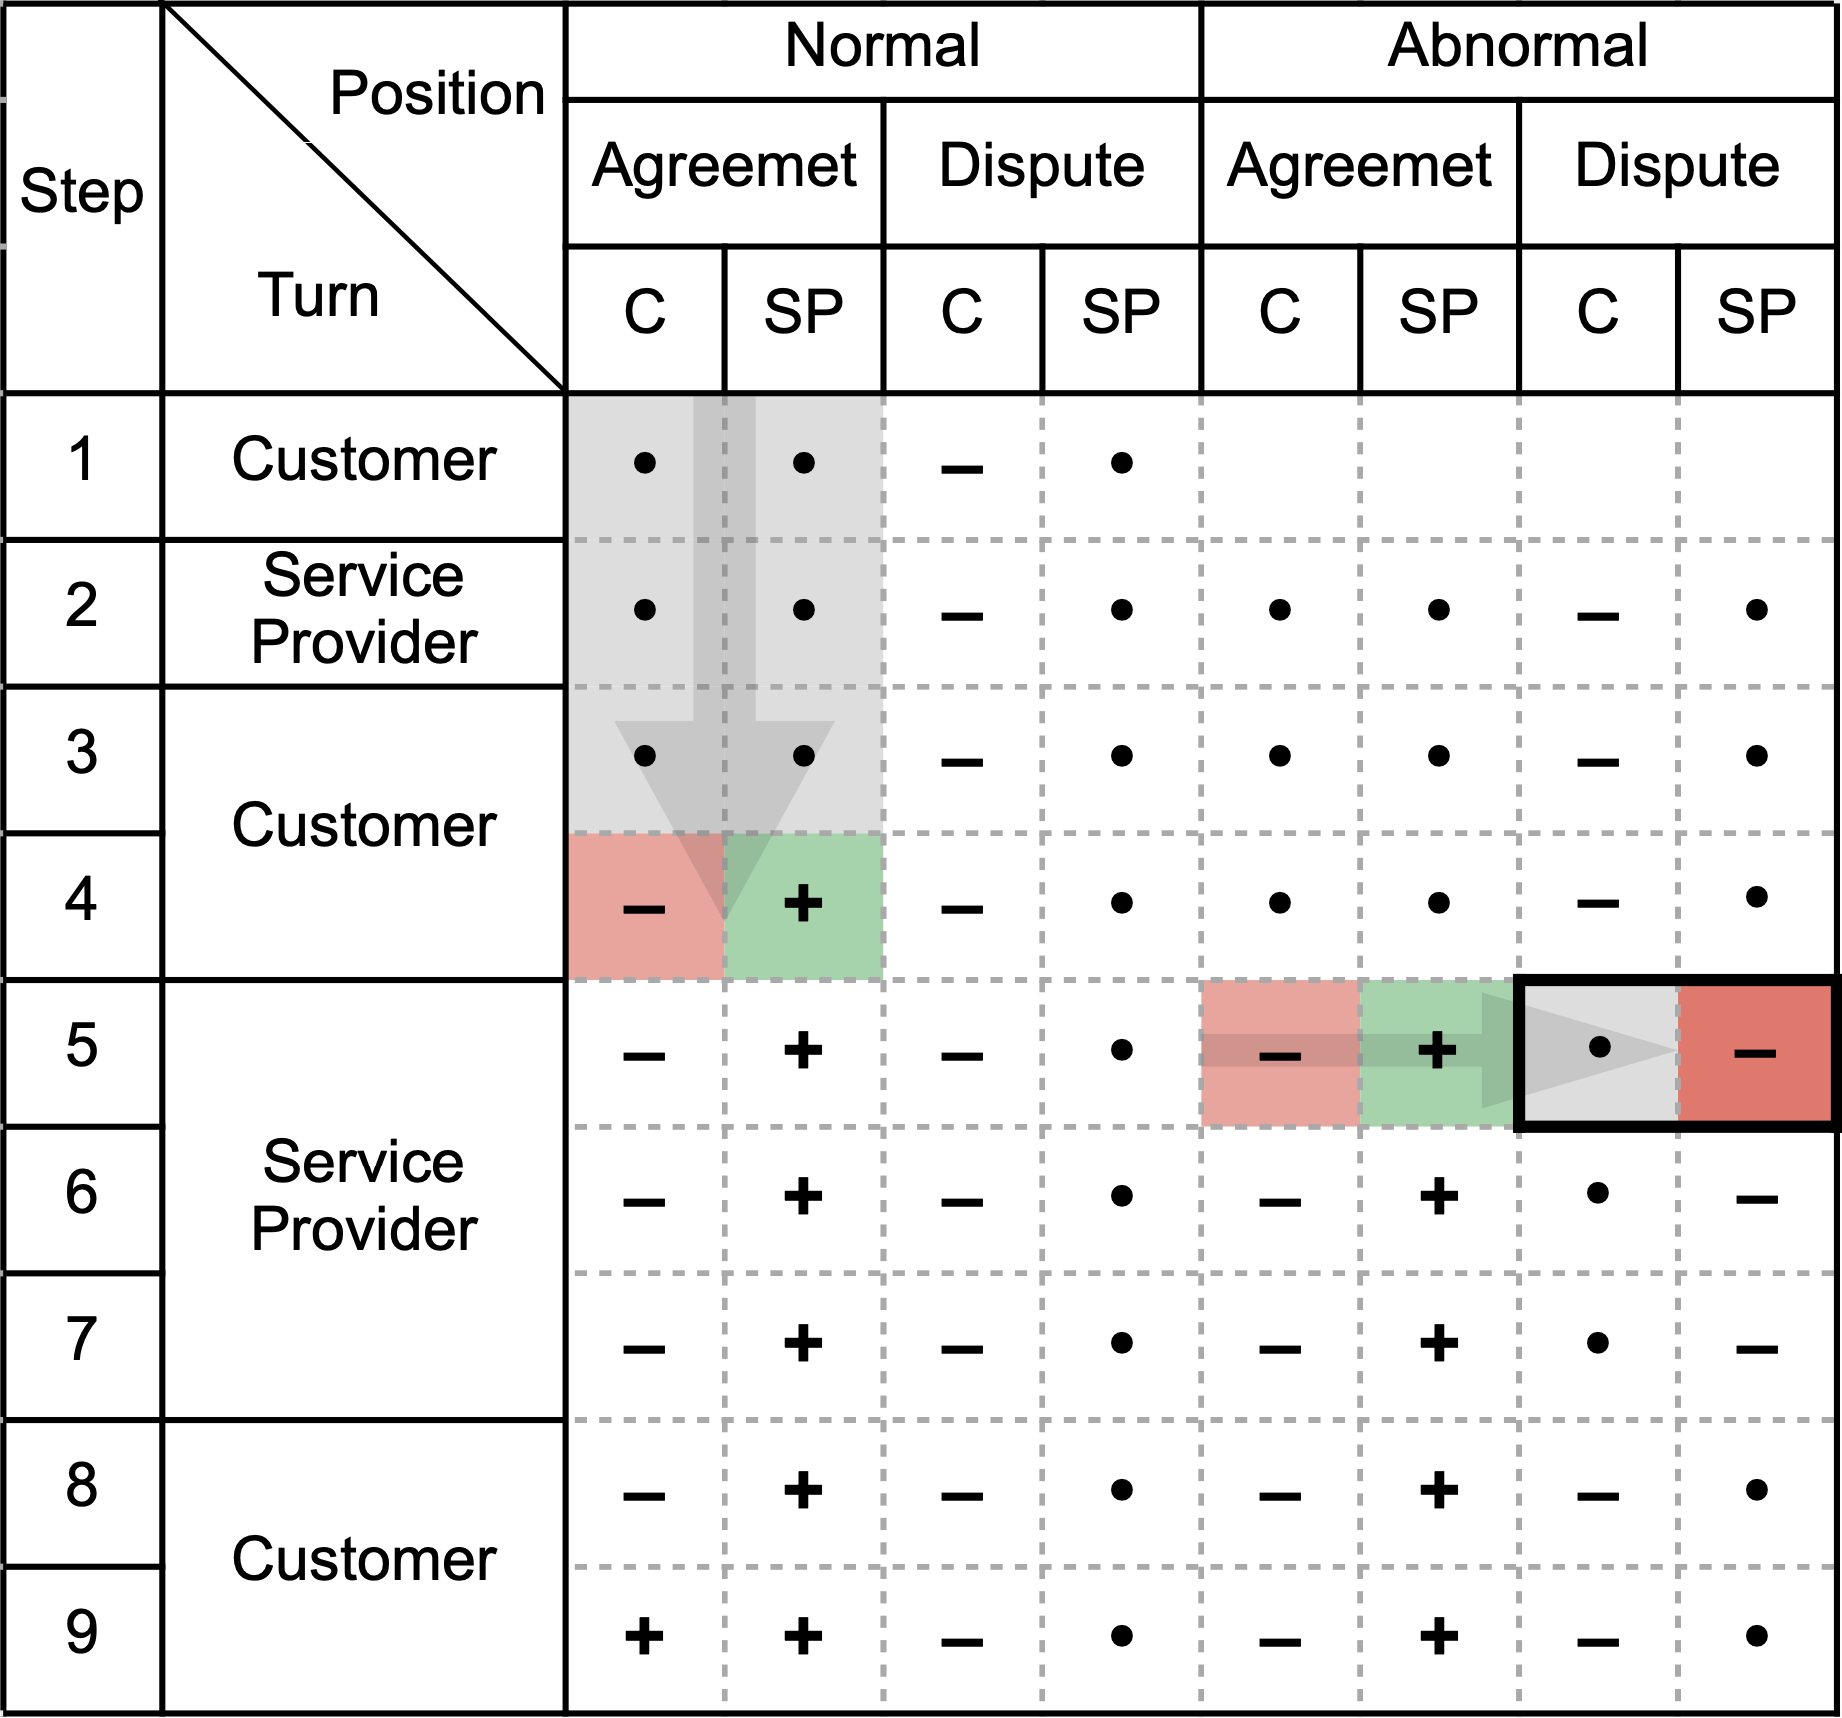
\includegraphics[width=\linewidth]{misbehaviour.png}
\centering
\caption{Transitions of positions in a scenario where the SP misbehaves by failing to perform the service and publish $\mathrm{PoP}$ after receiving payment. This leads to the customer initiating a dispute.}
\label{fig:misbehaviour}
\end{figure}

In the second scenario (Figure~\ref{fig:misbehaviour}), (1) the customer initialises the transaction and delivers the material to the SP, (2) who validates the material and publishes the Proof of Delivery ($\mathrm{PoD}$) on blockchain. (3) The customer validates the existence of the PoD on the blockchain, and (4) pays for the transaction using one of the specified payment methods. (5) The SP misbehaves by not provisioning the service and consequently not publishing the Proof of Provision ($\mathrm{PoP}$) after receiving the payment. Once the agreed $\mathrm{T}_\mathrm{provide}$ deadline has passed, the position moves to the Abnormal column and the customer is in a disadvantaged position and the SP is in an advantaged position. However, the customer is justified in starting a dispute by collecting all the evidence, i.e. Proof of Delivery ($\mathrm{PoD}$) from the message board, payment $\mathrm{recipt}$, and submitting it to the dispute resolution service. The customer is likely to win this dispute as the SP cannot prove the timely publication of $\mathrm{PoP}$. This scenario results in a neutral outcome for the customer and a disadvantaged outcome for the SP.


\section{Experiments}\label{sec:experiments}

The prototype of our protocol has been developed using a number of technologies designed to ensure anonymity and security:
\begin{itemize}
\begin{sloppypar}
  \item \textbf{Anonymous Payments:} Use of the Monero blockchain for secure transactions.
\end{sloppypar}
  \item \textbf{Storage Network:} Powergate serves as an interface for Filecoin and IPFS, facilitating decentralized storage.
  \item \textbf{Message Board:} The Ethereum blockchain, accessed via a local development version Truffle Ganache and Solidity, acts as a public ledger.
  \item \textbf{Customer and SP Interface:} A client-side web application built with \texttt{React.js} and \texttt{web3.js}, with \texttt{MetaMask} for Ethereum transactions and \texttt{monero-wallet-cli} for Monero interactions.
\end{itemize}

We used the following tools to create the experiment:
\texttt{monerod} and \texttt{monero-wallet-cli} - v0.18.1.2; \texttt{Powergate} - v2.6.2; \texttt{Ganache} - v7.5.0; \texttt{Solidity} - v0.8.17; \texttt{ReactJS} - v18.0.25; \texttt{web3.js} - v1.8.1; \texttt{crypto-js} - v4.1.1.

For simplicity, all components run on one physical machine; and all processes are managed by Docker. 
Moreover, Powergate is configured to use local Filecoin and IPFS networks.
For the Ethereum blockchain, we use Truffle Ganache, which is a local Ethereum blockchain for development and testing purposes. 
Monero is configured to use the public stage network.
We assume that the service provider offers only one type of service at a fixed public price, so we omit the service type and price from the protocol.

The prototype is available at \url{https://anonser.stan.bar}. The source code is available at \url{https://github.com/stanbar/anonser}.

In preparation for the experiment, both the customer and the SP set up their Monero wallets using the \texttt{monero-wallet-cli}. The SP deploys the smart contract to the Ethereum blockchain with the \texttt{truffle migrate --network development} command, and the web application is then configured to interact with this newly deployed contract.
The customer acquires test Monero funds from a Faucet service and configures their wallet to generate transaction proofs, essential for dispute resolution.
With preparations complete, the experiment proceeds as follows:

\begin{enumerate}
  \setcounter{enumi}{-1}
  \item \textbf{Setup:} The customer begins by creating a new provision in the webapp, which generates a unique ECDSA keypair and provisionID. The corresponding QR code is printed and attached to the parcel for delivery.
  
  \item  \textbf{Package Delivery:}  The parcel is delivered to the SP through a chosen delivery method, such as a secure drop box or locker service. Upon receipt, the SP scans the QR code to retrieve the provisionID and customer's public key. Since (in this experiment) the provision was not paid in cash, the SP generates a unique Monero payment address using \texttt{monero-wallet-cli integrated\_address}. As a result, the PoD is prepared.

  \item \textbf{Proof of Delivery:} Then, the SP submits the PoD to the Ethereum blockchain using the MetaMask interface.

    \item \textbf{Get Proof of Delivery:} The customer checks the transaction status on the Ethereum blockchain by calling \texttt{getProvision} with arguments \texttt{customerPubKey} and \texttt{provisionID}

    \begin{sloppypar}
    \item \textbf{Payment:} The customer sends the payment (using \texttt{monero-wallet-cli transfer}) to the \texttt{paymentAddress} specified in the smart contract and stores the payment receipt using \texttt{monero-wallet-cli get\_tex\_key <tx-id>}.
    \end{sloppypar}
  
    \item \textbf{Provision of Service:} Upon payment confirmation, the SP provides the service, resulting in a \texttt{result.pdf} file.

  \item \textbf{Upload result:} This file is uploaded to IPFS and Filecoin, granting the SP a \texttt{cid}, \texttt{dealID}, and \texttt{minerID}.

  \item \textbf{Proof of Provision:} A PoP is submitted to the Ethereum blockchain by the SP.

    \item \textbf{Get Proof of Provision:} Meanwhile, the customer subscribes to Ethereum and waits for the SP to publish the PoP.


  \item \textbf{Download result:} Upon noticing the PoP, the customer retrieves the result using either one of the public gateways\footnote{IPFS Public Gateway Checker, \url{https://ipfs.github.io/public-gateway-checker/}, (last visited Jan. 04, 2023)} like \url{https://cf-ipfs.com/ipfs/<cid>} or Lotus network using \texttt{lotus} \texttt{retrieve} \texttt{<cid>} \texttt{<minerID>}. The result is then decrypted using the customer's previously stored private key. If the customer is satisfied with the service the protocol ends; otherwise, the customer may initiate a dispute process.
  
\end{enumerate}

\subsection{Results}

\paragraph{Fairness}
As shown in Section~\ref{sec:proofs} the protocol is fair. This was achieved through an undeniable handshake mechanism, where the SP first commits to the package delivery and service deadlines by publishing the PoD (as outlined in step 2). The customer then acknowledges this commitment and accepts the terms by proceeding with the payment for the service (step 3).

Once payment is confirmed, the SP is incentivized to fulfill the service obligations. The SP must deliver the service and publish both the results and the PoP before the agreed deadline (step 7). Failure to do so allows the customer, equipped with all necessary evidence, to initiate a dispute and potentially penalize the SP. This mechanism ensures that rational parties are motivated to adhere to the protocol.

The protocol also ensures non-repudiation without the need for a TTP by employing blockchain technology and digital signatures. The blockchain provides a transparent and immutable record, ensuring that any changes to the smart contract's state are publicly visible and can only be made by the SP.


\paragraph{Anonymity}
\begin{sloppypar}
Anonymity was ensured by breaking the link between personal data and transactional elements, including materials, payments, and communications. We used anonymous payment methods such as cash and privacy-centric cryptocurrencies like Monero, to conceal transactional details. Furthermore, we leveraged decentralized storage networks like IPFS and Filecoin, which facilitate the anonymous storage and retrieval of data. This approach guaranteed that, in the dispute-free transaction, customer interactions with the protocol remained confidential at every stage.

Depending on the specific use case, the anonymity of the customer may be lost if the resolution of the dispute (e.g. by the police) involves the identification of the customer. However, even if the Dispute Resolution Service identifies the customer, the customer's identity won't be disclosed to the SP, which is the main goal of the protocol.

To maintain anonymity in the event of a dispute,
Online Dispute Resolution systems~\cite{allenGovernanceBlockchainDispute2019, lingwallShouldCodeBe2019} such as  Kleros~\cite{bergollaKlerosSociolegalCase2022, nappertDecentralizedJusticeReinventing2020, gudkovCrowdArbitrationBlockchain2020} should be used, where only the customer's pseudonym is revealed and anonymous evidence can be provided in zero-knowledge proofs. We discuss this further in Section~\ref{sec:decentralised-justice}.
\end{sloppypar}

\paragraph{Provable Results Availability}\label{sec:provable-results-availability}
The availability of the result is guaranteed by the usage of Filecoin~\cite{protocollabsFilecoinDecentralizedStorage2017}, which operates as an incentivization layer on top of IPFS. Filecoin enhances content availability by economically penalizing the lack of proof of content storage~\cite{filecoinSlashing}.

In our protocol, the SP is responsible for uploading the result to both the IPFS and Filecoin networks (utilizing Powergate), which ensures free access to the results under normal operational circumstances. This dual-network approach also ensures high availability of the results, even if the SP ceases to host the content on their node.

\paragraph{Costs}
The deployment and operation of smart contracts on the Ethereum blockchain incur gas fees, which are proportional to the computational resources required for transaction execution. The following outlines the gas consumption and associated costs for each operation within our protocol, based on the testnet metrics, which are analogous to the mainnet:

The cost of gas is denominated in ETH, and the price per unit of gas at the time of the experiment (January 3, 2023) was 0.000000002227 ETH/gas, with the ETH price being \$1,261.97 USD\footnote{Etherscan Gas Tracker, \url{https://etherscan.io/gastracker}}. The customer is responsible only for covering the payment transaction fee. For transactions using Monero, the fee was approx. 0.000304 XMR at the time of the experiment, with the price of Monero being \$150 USD per XMR\footnote{Cryptocurrency statistics, \url{https://bitinfocharts.com}}.

The incurred costs are summarized in Table~\ref{table:costs}:

\begin{table}
\caption{Incurred Costs for Protocol Operations}
\centering
\label{table:costs}
\begin{tabular}{lrr}
\hline
\textbf{Operation}            & \textbf{Gas Units} & \textbf{Cost (USD)} \\
\hline
Smart Contract Deployment     & 1,456,577          & 4.09                \\
Proof of Delivery             & 129,649            & 0.29                \\
Payment (Monero)              & -                  & 0.0456              \\
Proof of Provision            & 149,130            & 0.33                \\
\hline
\end{tabular}
\end{table}

Additionally, our protocol's interaction with the Filecoin network introduces costs in FIL cryptocurrency for data storage and retrieval. These costs are determined through market-driven deals with miners. Deal prices, quoted in FIL, are influenced by various factors including data size, storage duration, and miner policies. The dynamic nature of these parameters means that costs can fluctuate, making precise predictions challenging. However, for our experiment, we leveraged Filecoin's reputation-based incentivisation layer to publish deals at no cost\footnote{Filecoin, Filecoin Plus Overview, \url{https://docs.filecoin.io/store/filecoin-plus/overview/}, (last visited Jan. 04, 2023)}.

\paragraph{Performance Evaluation Metrics}

To provide a comprehensive performance evaluation of our protocol, we have analyzed the following metrics for each of the blockchain networks, as summarized in Table~\ref{table:performance}:

\begin{table}[h!]
\centering
\caption{Performance Evaluation Metrics}
\label{table:performance}
\begin{tabular}{lrrr}
\hline
\textbf{Network}     & \textbf{Block Time} & \textbf{Tx Throughput} & \textbf{Tx Latency} \\ \hline
Ethereum             & 13-15 sec       & 15-30 TPS                       & \textasciitilde{}6 min      \\
Monero               & \textasciitilde{}2 min & \textasciitilde{}4 TPS             & \textasciitilde{}20 min \\
Filecoin             & 30 sec & N/A\footnotemark{}            & 5-10 min  \\ 
\hline
\end{tabular}
\end{table}

\footnotetext{The network is optimized for storage operations rather than transaction processing, with the throughput being primarily dependent on the storage and retrieval deal proposals.}


These metrics are crucial for understanding the scalability and efficiency of the blockchain networks in question and provide insight into their suitability for various applications within our protocol.
\section{Discussion}
\label{sec:discussion}

\subsection{Dispute Resolution Service}\label{sec:decentralised-justice}

\begin{sloppypar}
The central challenge in achieving a Web3-compliant system lies in the centralization of dispute resolution services~\cite{ethereumWhatWeb3Why2023}. To address this, we consider two potential solutions: the integration of blockchain-based dispute resolution systems and the development of mechanisms to ensure the infeasibility of incorrect service provision.
\end{sloppypar}

Blockchain-based dispute resolution platforms such as  Kleros~\cite{bergollaKlerosSociolegalCase2022, nappertDecentralizedJusticeReinventing2020, gudkovCrowdArbitrationBlockchain2020}, Themis~\cite{mengThemisDecentralizedEscrow2019}, Aragon Court~\cite{AragonWhitepaper2023,aragonDecentralizedDisputeResolution}, LTO Network~\cite{ltonetworkNextGenBlockchainB2B}, and other Online Dispute Resolution (ODR) systems~\cite{allenGovernanceBlockchainDispute2019, lingwallShouldCodeBe2019} offer a promising direction. These systems could employ a pool of field experts who, in the event of a dispute, would examine the smart contract, the proofs ( $\mathrm{PoD}$, $\mathrm{PoP}$, payment $\mathrm{receipt}$) and provide verdicts. Expert participation and honest verdicts are encouraged through a system of fees, stakes and rewards. At the time of writing Kleros is the most successful platform for resolving consumer disputes in e-commerce or collaborative economy. It has received funding from the Commission's European Innovation Council~\cite{CommissionEuropeanInnovation2020}. The protocol claims to have resolved 1645 disputes, employing 716 jurors and rewarding them with 401 ETH~\cite{KlerosHomepage}. Kleros allows integration with new protocols and we leave it to future work.

The second, more visionary approach involves ensuring service correctness through computational proofs, such as zkSNARKs~\cite{ben-sassonSNARKsVerifyingProgram2013}, which could validate the accuracy of services that are fully computable. This method, however, faces significant challenges in representing physical materials like blood or saliva digitally—a prerequisite for end-to-end service verification and the elimination of disputes.

\subsection{Self-sovereign Identities}
In our exploration of privacy-preserving protocols, we encountered regulatory requirements that mandate the linking of diagnostic results to patient identities, as is the case in Poland~\cite{ministerstwozdrowiaRegulationMinisterHealth2006}. Such regulations present a direct challenge to our protocol's objective of anonymity.

The concept of self-sovereign identities (SSIs) and verifiable claims offers a potential resolution~\cite{muhleSurveyEssentialComponents2018}. Under this system, a trusted entity, such as a government body, could issue a one-time, verifiable claim to the customer. Service providers would accept this claim as valid identification, linking diagnostic results to a Decentralized Identifier (DID) that holds no personal data. While this ensures the SP cannot deduce the customer's identity, the DID could be traced back to the individual by the issuing authority if necessary.

Given the early stage of SSI technology and its current lack of governmental adoption, we recognize the need for further research and development in this area.

\subsection{Formal Verification}\label{sec:formal-verification}
Following the work of~\cite{birjoveanuFormalVerificationMultiparty2022}, the security analysis of our protocol could be improved by using automatic formal verification tools, such as AVISPA~\cite{armandoAVISPAToolAutomated2005}. This process would involve formulating the protocol in the High-Level Protocol Specification Language (HLPSL)~\cite{chevalierHighLevelProtocol2004}, followed by its translation into AVISPA's intermediate format. Subsequently, AVISPA's tools would rigorously assess the protocol's adherence to established security properties through automated theorem proving and model checking techniques.


\subsection{Ethical and Regulatory Considerations}

The core objective of our protocol is to facilitate anonymous access to services without necessitating the disclosure of personal information, which naturally raises concerns regarding regulatory compliance, particularly with Know Your Customer (KYC), Anti-Money Laundering (AML), and regulations concerning Politically Exposed Persons (PEP).

Our approach is explicitly designed to integrate with services that inherently comply with applicable local and international regulations. This integration ensures that while our protocol itself operates under the premise of anonymity, it does not facilitate illegal activities or contravene established legal frameworks. Specifically, the services that would utilize our protocol are those not primarily involved in financial transactions or money transmission, thereby not falling directly under the stringent requirements of financial regulations such as KYC and AML.

We acknowledge that the use of anonymous payment methods, such as cryptocurrencies like Monero, might raise suspicions due to their common association with privacy and potential misuse. However, it is important to note that Monero is just one of several anonymous payment methods that could be utilized with our protocol. Our design is versatile enough to support a variety of payment mechanisms, both blockchain-based and non-blockchain-based.

\begin{sloppypar}
For instance, we could employ the Ethereum network and utilize privacy mixers to ensure private payments. Nevertheless, privacy mixers have drawn scrutiny from regulators because they are increasingly used by malicious actors to obscure the origins of funds illicitly. A notable example is Tornado Cash, the largest privacy mixer to date, which has faced sanctions across significant portions of the Ethereum network. Ongoing research into compliant privacy mixers, such as the Voluntary Reveal Approach proposed in~\cite{dotanHazeCompliantPrivacy2023}, seeks to address these concerns. This approach involves Proofs of Innocence required before a user can access the system and incorporates oracles for monitoring sanctioned addresses—currently maintained on the Ethereum blockchain by Chainalysis~\cite{ChainalysisOracleSanctions}.
\end{sloppypar}

\section{Conclusions}\label{sec:conclusion}

This study has been dedicated to the development of a protocol that facilitates the provision of services while preserving the anonymity of the user. Our protocol is particularly applicable to services requiring a high degree of confidentiality, such as genetic testing, paternity determination, and anonymous legal consultation.

We found that the current state of the art was not sufficient to achieve this goal, so we have designed and implemented a novel protocol that ensures user anonymity, fairness in service delivery, and a mechanism for dispute resolution without the need for a trusted third party. This protocol leverages anonymous payment systems, such as cash or privacy-focused cryptocurrencies, and utilizes peer-to-peer networks for the dissemination of service results.

\begin{sloppypar}
Through rigorous definition and analysis, we have demonstrated that our protocol meets the criteria for fairness, as outlined in Definition~\ref{def:fairness}. It does so by systematically publishing proofs of delivery, payment, and provisioning, ensuring a transparent and equitable process for all parties involved.
\end{sloppypar}

In closing, we have pinpointed several avenues for future enhancement, including the integration of decentralized dispute resolution systems, the application of self-sovereign identity (SSI) frameworks, and the exploration of anonymous physical delivery methods. These areas present exciting opportunities for further research and development towards the realization of fully anonymous service provision in the digital age.

\paragraph{Data availability}
No data was used for the research described in the article.
The prototype is available at \url{https://anonser.stan.bar}. 
The source code is available at \url{https://github.com/stanbar/anonser}.

\section*{Declarations}

\paragraph{Conflict of interest} The authors declare that they have no competing interests. The authors certify that they have no affiliations with or involvement in any organisation or entity with any financial interest or non-financial interest in the subject matter or materials discussed in this manuscript.

\paragraph{Ethical approval} This article does not contain any studies with human participants or animals performed by any of the authors


\appendix

\begin{sloppypar}
\section{Proof of fairness}\label{app:proof-of-fairness}
Below we describe each step and the reasoning behind the outcome position.
We use the notation introduced in Section~\ref{sec:fairness-model} to analyse each position in the protocol and to show the fairness of the protocol.

\newcommand{\AgreeablePath}{Agreeable path:}
\newcommand{\DisputePath}{The customer starts a dispute:}
\newcommand{\Fairness}{Fairness:}
\newcommand{\CustomerTurn}[0]{\expandafter\MakeUppercase customer turn:}
\newcommand{\SPTurn}[0]{\sp{} turn:}

\newcommand{\CanFollowToOne}[2]{The #1 can follow the protocol to the non-disadvantaged position #2}
\newcommand{\CanDoNothing}[1]{The #1 can do nothing and always ends up in the non-disadvantaged position}
\newcommand{\CanDoAnything}[1]{The #1 can do anything and always ends up in the non-disadvantaged position}
\newcommand{\Pos}[4]{$\operatorname{\sigma_{#1, #2, #3} = #4}$}
\newcommand{\WinForTheSameReason}[1]{The #1 wins the dispute for the same reason}
\newcommand{\LoseForTheSameReason}[1]{The #1 loses the dispute for the same reason}
\newcommand{\ActedAbnormallyThen}[1]{The #1 acted abnormally, then:}
\newcommand{\CustomerPaidButDidntGetResult}{The customer ends up in a disadvantageous position, because he has paid in advance, but hasn't received the result}
\newcommand{\SpReceivedThePayment}{The SP ends up in the advantageous position, having received the payment}

\newcommand{\CustomerLosesBeforePayment}{The customer loses the dispute because the SP is not obliged to do anything until the transaction is paid}
\newcommand{\CustomerLosesBeforePoP}{The customer loses the dispute because the SP is still able to publish the PoP within the agreed timeframe}

\newcommand{\RemainsIn}[2]{The #1 remains in the #2 position}

\subsubsection*{Step 1. \CustomerTurn{} Package delivery}\label{step-1-deliver-package}

The protocol starts when the customer correctly completes the first step of the protocol, i.e. delivers the package to the SP. 

The case where the customer does not deliver the package is not considered as it is not part of the protocol.

\begin{itemize}
\item \AgreeablePath
  \begin{itemize}
    \item \Pos{1}{c}{\normal}{\neutral}, the customer risked his materials but did not pay for the transaction and therefore ends up in a neutral position (see Assumption 10. in Section \ref{sec:assumptions}).
    \item \Pos{1}{s}{\normal}{\neutral}, the SP ends up in a neutral position as she did not spend any resources and the package did not bring her any value.
  \end{itemize}
\item \DisputePath
  \begin{itemize}
    \item \Pos{1}{c}{\dispute}{\minus}, \CustomerLosesBeforePayment{}.
    \item \Pos{1}{s}{\dispute}{\neutral}, \WinForTheSameReason{SP}.
  \end{itemize}
\end{itemize}

\Fairness

\begin{itemize}
  \item \CanFollowToOne{customer}{\Pos{1}{c}{n}{\neutral}}
  \item \CanDoNothing{SP}
\end{itemize}

\subsubsection*{Step 2. \SPTurn{} Proof of Delivery}\label{step-2-proof-of-delivery}

The SP publishes the PoD, then:

\begin{itemize}
  \item \AgreeablePath
    \begin{itemize}
      \item \Pos{2}{c}{\normal}{\neutral}, the customer remains in the neutral position as the PoD allows him to pay for the transaction but does not oblige him to do anything.
      \item \Pos{2}{s}{\normal}{\neutral}, the SP remains in the neutral position as the package has not brought her any value and she has not spent any resources to provide the service.
    \end{itemize}

  \item \DisputePath
    \begin{itemize}
      \item \Pos{2}{c}{\dispute}{\minus}, \CustomerLosesBeforePayment{}.
      \item \Pos{2}{s}{\dispute}{\neutral}, \WinForTheSameReason{SP}.
    \end{itemize}
\end{itemize}

\ActedAbnormallyThen{\sp}

\begin{itemize}
\item \AgreeablePath
  \begin{itemize}
    \item \Pos{2}{c}{\abnormal}{\neutral}, the customer remains in the neutral position as he is not obliged\footnote{By not obliged we understand the situation where a party does not risk any resources by not taking the action} to agree with the incorrect $\mathrm{PoD}$.
    \item \Pos{2}{s}{\abnormal}{\neutral}, the SP remains in the neutral position as the package has not brought her any value and she has not spent any resources to provide the service.
  \end{itemize}
\item \DisputePath
  \begin{itemize}
    \item \Pos{2}{c}{\abdispute}{\minus}, \CustomerLosesBeforePayment{}, not even to publish correct $\mathrm{PoD}$.
    \item \Pos{2}{s}{\abdispute}{\neutral}, \WinForTheSameReason{SP}.
  \end{itemize}
\end{itemize}

\Fairness

\begin{itemize}
  \item \CanDoAnything{SP}.
  \item customer can either wait (if the SP is following the protocol) or abandon the transaction (if the SP is acting abnormally). In both cases the customer ends up in a non-disadvantaged position \Pos{2}{c}{\normal}{\neutral} or \Pos{2}{c}{\abnormal}{\neutral}.
\end{itemize}


\subsubsection*{Step 3. \CustomerTurn{} Get Proof of Delivery}\label{step-3-get-proof-of-delivery}

The customer got the \PoD, then:

\begin{itemize}
\item \AgreeablePath
  \begin{itemize}
    \item \Pos{3}{c}{\normal}{\neutral}, \RemainsIn{customer}{neutral}.
    \item \Pos{3}{s}{\normal}{\neutral}, \RemainsIn{SP}{neutral}.
  \end{itemize}
\item \DisputePath
  \begin{itemize}
    \item \Pos{3}{c}{\dispute}{\minus}, \CustomerLosesBeforePayment{}.
    \item \Pos{3}{s}{\dispute}{\neutral}, \WinForTheSameReason{SP}.
  \end{itemize}
\end{itemize}

\ActedAbnormallyThen{Customer}

\begin{itemize}
\item \AgreeablePath
  \begin{itemize}
    \item \Pos{3}{c}{\abnormal}{\neutral}, \RemainsIn{customer}{neutral}.
    \item \Pos{3}{s}{\abnormal}{\neutral}, \RemainsIn{SP}{neutral}.
  \end{itemize}
\item \DisputePath
  \begin{itemize}
    \item \Pos{3}{c}{\abdispute}{\minus}, \CustomerLosesBeforePayment{}.
    \item \Pos{3}{s}{\abdispute}{\neutral}, \WinForTheSameReason{SP}.
  \end{itemize}
\end{itemize}

\Fairness

\begin{itemize}
  \item \CanFollowToOne{customer}{\Pos{3}{c}{\normal}{\neutral}}.
  \item \CanDoNothing{SP}.
\end{itemize}



\subsubsection*{Step 4. \CustomerTurn{} Payment}

The customer paid the transaction, then:

\begin{itemize}
\item \AgreeablePath
  \begin{itemize}
    \item \Pos{4}{c}{\normal}{\minus}, the customer has paid in advance.
    \item \Pos{4}{s}{\normal}{\plus}, the SP has received the payment but has not spent his resources yet.
  \end{itemize}
\item \DisputePath
  \begin{itemize}
    \item \Pos{4}{c}{\dispute}{\minus}, \CustomerLosesBeforePoP{}.
    \item \Pos{4}{s}{\dispute}{\neutral}, \WinForTheSameReason{SP}.
  \end{itemize}
\end{itemize}

\ActedAbnormallyThen{Customer}

\begin{itemize}
\item \AgreeablePath
  \begin{itemize}
    \item \Pos{4}{c}{\abnormal}{\neutral}, the customer ends up in the neutral position as he has not spent his funds.
    \item \Pos{4}{s}{\abnormal}{\neutral}, the SP ends up in the neutral position as she neither received the payment nor spent her resources.
  \end{itemize}
\item \DisputePath
  \begin{itemize}
    \item \Pos{4}{c}{\abdispute}{\minus}, \CustomerLosesBeforePayment{}.
    \item \Pos{4}{s}{\abdispute}{\neutral}, \WinForTheSameReason{SP}.
  \end{itemize}
\end{itemize}

\Fairness

\newcommand{\CustomerRiskTemporaryDisadvantagedPosition}[1]{The customer, following the 9th assumption described in Section~\ref{sec:assumptions}, risks the temporary disadvantaged position #1 in favour of a later better position \Pos{9}{s}{\normal}{\plus}; in the meantime, he can get out of the disadvantaged position if the SP misbehaves in any of the following steps.}

\begin{itemize}
  \item \CustomerRiskTemporaryDisadvantagedPosition{\Pos{4}{c}{\normal}{\minus}}
  \item \CanDoNothing{SP}.
\end{itemize}



\subsubsection*{Step 5. \SPTurn{} Provision of service}

The \sp{} did the provision of service, then:

\begin{itemize}
\item \AgreeablePath
  \begin{itemize}
    \item \Pos{5}{c}{\normal}{\minus}, \RemainsIn{Customer}{disadvantaged} as he hasn't received the result.
    \item \Pos{5}{s}{\normal}{\plus}, \RemainsIn{\sp}{advantaged} as she has received the payment.
  \end{itemize}
\item \DisputePath
  \begin{itemize}
    \item \Pos{5}{c}{\dispute}{\minus}, \CustomerLosesBeforePoP{}.
    \item \Pos{5}{s}{\dispute}{\neutral}, \WinForTheSameReason{SP}.
  \end{itemize}
\end{itemize}

\ActedAbnormallyThen{\sp}

\begin{itemize}
\item \AgreeablePath
  \begin{itemize}
    \item \Pos{5}{c}{\abnormal}{\minus}, \CustomerPaidButDidntGetResult{}. 
    \item \Pos{5}{s}{\abnormal}{\plus}, \SpReceivedThePayment{}.
  \end{itemize}
\item \DisputePath
  \begin{itemize}
    \item \Pos{5}{c}{\abdispute}{\neutral} The customer wins the dispute because the SP has not provided the service within the time agreed in the \PoD{}, and therefore the SP is unable to upload the result and publish the \PoP{} on time.
    \item \Pos{5}{s}{\abdispute}{\minus}, \LoseForTheSameReason{SP}.
  \end{itemize}
\end{itemize}

\Fairness
\newcommand{\SPCanDoBothButFollowIsSafe}[1]{The SP can follow the protocol and move to the advantaged position \Pos{#1}{s}{\normal}{\plus}, or act abnormally (not provide the service) and also move to the advantaged position \Pos{#1}{s}{\abnormal}{\plus}; however, the second option puts her at risk of terminating the protocol at \Pos{#1}{s}{\abdispute}{\minus} if the customer is rational and starts a dispute; hence, the SP should choose the first option}

\begin{itemize}
  \item \CustomerRiskTemporaryDisadvantagedPosition{\Pos{5}{c}{\normal}{\minus}}
  \item \SPCanDoBothButFollowIsSafe{5}.
\end{itemize}

\subsubsection*{Step 6. \SPTurn{} Upload result}\label{step-6-publication-of-results}

The SP uploaded the result on time, then:

\begin{itemize}
\item \AgreeablePath
  \begin{itemize}
    \item \Pos{6}{c}{\normal}{\minus}, \RemainsIn{Customer}{disadvantaged} as he has not received the result.
    \item \Pos{6}{s}{\normal}{\plus}, \RemainsIn{SP}{advantaged} as she has received the payment.
      \end{itemize}
\item \DisputePath
  \begin{itemize}
    \item \Pos{6}{c}{\dispute}{\minus}, \CustomerLosesBeforePoP{}.
    \item \Pos{6}{s}{\dispute}{\neutral}, \WinForTheSameReason{SP}.

  \end{itemize}
\end{itemize}

\ActedAbnormallyThen{\sp}

\begin{itemize}
\item \AgreeablePath
  \begin{itemize}
    \item \Pos{6}{c}{\abnormal}{\minus}, \CustomerPaidButDidntGetResult{}.
    \item \Pos{6}{s}{\abnormal}{\plus}, \SpReceivedThePayment{}.
  \end{itemize}
\item \DisputePath
  \begin{itemize}
    \item \Pos{6}{c}{\abdispute}{\neutral}, the customer wins the dispute because the SP has not uploaded the service within the time agreed in the \PoD{} and the SP will not be able to publish the \PoP{} on time.
    \Pos{6}{s}{\abdispute}{\minus}, \LoseForTheSameReason{SP}.
  \end{itemize}
\end{itemize}

\Fairness

\begin{itemize}
  \item \CustomerRiskTemporaryDisadvantagedPosition{\Pos{6}{c}{\normal}{\minus}}
  \item \SPCanDoBothButFollowIsSafe{6}.
\end{itemize}

\subsubsection*{Step 7. \SPTurn{} Proof of provision}\label{step-7-publication-of-proof-of-provision}

The SP published \PoP{} on time, then:

\newcommand{\CustomerLosesBecauseSPCanProveBeingCorrect}{the customer loses the dispute as the \sp{} has published all evidences to prove her correct behaviour}

\begin{itemize}
  \item \AgreeablePath
    \begin{itemize}
      \item \Pos{7}{c}{\normal}{\minus}, the customer has not received the result. Therefore, he remains in a disadvantaged position. 
      \item \Pos{7}{s}{\normal}{\plus}, the SP has published all the evidence to prove her correct behaviour, so she remains in an advantageous position for the rest of the protocol.
    \end{itemize}
  \item \DisputePath
    \begin{itemize}
      \item \Pos{7}{c}{\dispute}{\minus}, \CustomerLosesBecauseSPCanProveBeingCorrect{}.
      \item \Pos{7}{s}{\dispute}{\plus}, \WinForTheSameReason{SP}.
    \end{itemize}
\end{itemize}

\ActedAbnormallyThen{\sp}

\begin{itemize}
\item \AgreeablePath
  \begin{itemize}
    \item \Pos{7}{c}{\abnormal}{\minus}, \CustomerPaidButDidntGetResult{}.
    \item \Pos{7}{s}{\abnormal}{\plus}, \SpReceivedThePayment{}.
  \end{itemize}
\item \DisputePath
  \begin{itemize}
    \item \Pos{7}{c}{\abdispute}{\neutral}, the customer wins the dispute because the SP did not publish the correct \PoP{} on time.
    \item \Pos{7}{s}{\abdispute}{\minus}, \LoseForTheSameReason{SP}.
  \end{itemize}
\end{itemize}

\Fairness

\begin{itemize}
  \item \CustomerRiskTemporaryDisadvantagedPosition{\Pos{7}{c}{\normal}{\minus}}
  \item \SPCanDoBothButFollowIsSafe{7}.
\end{itemize}


\subsubsection*{Step 8. \CustomerTurn{} Get Proof of Provision}\label{step-8-pull-proof-of-provision}

The customer got the \PoP{}, then:

\begin{itemize}
\item \AgreeablePath
  \begin{itemize}
    \item \Pos{8}{c}{\normal}{\minus}, the customer gets the \cid{}, but not the result yet.
    \item \Pos{8}{s}{\normal}{\plus}, \RemainsIn{\sp}{advantaged}.
  \end{itemize}
\item \DisputePath

  \begin{itemize}
    \item \Pos{8}{c}{\dispute}{\minus}, \CustomerLosesBecauseSPCanProveBeingCorrect{}.
    \item \Pos{8}{s}{\dispute}{\plus}, \WinForTheSameReason{SP}.
  \end{itemize}
\end{itemize}

\ActedAbnormallyThen{Customer}

\begin{itemize}
\item \AgreeablePath
  \begin{itemize}
    \item \Pos{8}{c}{\abnormal}{\minus}, the customer has paid for the transaction but does not have access to the $cid$ and therefore cannot get the result from the storage network.
    \item \Pos{8}{s}{\abnormal}{\plus}, \SpReceivedThePayment{}.
  \end{itemize}
\item \DisputePath
  \begin{itemize}
    \item \Pos{8}{c}{\abdispute}{\minus}, \CustomerLosesBecauseSPCanProveBeingCorrect{}
    \item \Pos{8}{s}{\abdispute}{\neutral}, \WinForTheSameReason{SP}.
  \end{itemize}
\end{itemize}


\Fairness

\begin{itemize}
  \item \CustomerRiskTemporaryDisadvantagedPosition{\Pos{8}{c}{\normal}{\minus}}
  \item \CanDoNothing{} \Pos{8}{s}{\normal}{\plus} or \Pos{8}{s}{\abnormal}{\plus}.
\end{itemize}

\subsubsection*{Step 9. \CustomerTurn{} Download result}\label{step-9-retrieval-of-results}

The customer downloaded the result, then:

\begin{itemize}
\item \AgreeablePath
  \begin{itemize}
    \item \Pos{9}{c}{\normal}{\plus}, The customer has received the result, therefore he finishes the protocol in an advantaged position.
    \item \Pos{9}{s}{\normal}{\plus}, \RemainsIn{\sp}{advantaged}.
  \end{itemize}
\item \DisputePath
  \begin{itemize}
    \item \Pos{9}{c}{\dispute}{\minus}, \CustomerLosesBecauseSPCanProveBeingCorrect{}.
    \item \Pos{9}{s}{\dispute}{\plus}, \WinForTheSameReason{SP}.
  \end{itemize}
\end{itemize}

\ActedAbnormallyThen{Customer}


\begin{itemize}
\item \AgreeablePath
  \begin{itemize}
    \item \Pos{9}{c}{\abnormal}{\minus}, the customer ends up in a disadvantaged position, as he ends up with the incorrect result.
    \item \Pos{9}{s}{\abnormal}{\plus}, the SP ends up in the advantageous position of having received the payment but not having spent his resources.
  \end{itemize}
\item \DisputePath
  \begin{itemize}
    \item \Pos{9}{c}{\abdispute}{\neutral}, the customer wins the case and ends up in the neutral position.
    \item \Pos{9}{s}{\abdispute}{\minus}, the SP loses the case and ends up in the disadvantaged position.
  \end{itemize}
\end{itemize}

\Fairness

\begin{itemize}
  \item \CanFollowToOne{Customer}{\Pos{9}{c}{\normal}{\plus}}.
  \item \CanDoNothing{} \Pos{9}{s}{\normal}{\plus} or \Pos{9}{s}{\abnormal}{\plus}. 
\end{itemize}

\end{sloppypar}


\bibliographystyle{spbasic}
\bibliography{bibliography-betterbibtex}
\end{document}